% (c)~2014 Claudio Carboncini - claudio.carboncini@gmail.com
% (c)~2014 Dimitrios Vrettos - d.vrettos@gmail.com
\chapter{La probabilità}
\section{Gli eventi}
L'esito del lancio di una moneta o di un dado, l'esito di un'estrazione del lotto, il sesso di un nascituro, la durata di una lampadina o di un computer sono esempi di fenomeni la cui realizzazione non può essere prevista con certezza; per questo vengono detti eventi casuali o aleatori (dal latino \emph{alea} che significa ``dado''). Spesso è necessario prendere decisioni in condizioni di incertezza: in quale università proseguire gli studi, decidere se fare il vaccino contro l'influenza, scommettere sulla vincita di una squadra, sull'uscita di una sequenza di numeri al gioco del lotto, \ldots{} \`E quindi fondamentale nei confronti di un fenomeno dall'esito incerto, poter identificare quali sono gli eventi che si possono verificare ed inoltre riuscire ad esprimere il proprio grado di fiducia nel verificarsi di tali eventi.

Quali sono gli eventi possibili per un dato fenomeno aleatorio? Supponiamo di lanciare un dado e di essere interessati alla faccia che si presenta dopo aver effettuato il lancio. Il lancio del dado rappresenta l'esperimento oggetto del nostro studio, l'uscita del numero 4 o l'uscita di un numero dispari sono detti \emph{eventi aleatori} o \emph{casuali}, in quanto sappiamo che si presenterà una delle facce, ma non sappiamo quale.

\begin{definizione}
Si chiama \emph{evento} il risultato di un \emph{fenomeno aleatorio}.
\end{definizione}

Se si considera la proposizione ``Oggi farà bel tempo'' è evidente che non è chiaro cosa si intende per bel tempo (senza pioggia? senza nuvole? con il sole?) né il luogo a cui ci si riferisce. Sarebbe meglio affermare per esempio ``Stamani a Milano ci sarà il sole''. \`E necessario quindi specificare con precisione l'evento che si considera in modo da essere sicuri se l'evento si è verificato o meno.

Nel lancio di un dado sono possibili sei risultati, espressi dai numeri da 1 a 6 e solo uno di essi si realizzerà.

Chiamiamo questi sei risultati \emph{eventi elementari} e indichiamo il loro insieme con 
\[\Omega =\{1\text{, }2\text{, }3\text{, }4\text{, }5\text{, }6\}.\]

\begin{definizione}
Si chiama \emph{spazio degli eventi}, l'insieme di tutti gli esiti possibili del fenomeno considerato. Tale insieme viene indicato con $\Omega$.
\end{definizione}

L'insieme $\Omega$ non esaurisce la totalità degli eventi collegati al lancio del dado; non comprende per esempio l'evento $P=\text{numero pari}$ o l'evento $M=\text{numero minore di }3$. Tuttavia $\Omega$ permette di rappresentare qualsiasi evento come suo particolare sottoinsieme.

\begin{definizione}
Si chiama \emph{evento elementare} ogni elemento dell'insieme $\Omega$, mentre \emph{evento composto} un sottoinsieme qualsiasi di $\Omega$.
\end{definizione}

Estraiamo una carta da un mazzo di 52 carte e consideriamo i seguenti eventi: ``uscita di un asso di cuori'' e ``uscita di un re''. Qual è la differenza fra questi due eventi? Il primo dei due è un evento elementare, mentre l'altro è un evento formato da quattro eventi elementari (tutti i possibili re presenti nel mazzo) e quindi è un evento composto.

Sono esempi di eventi composti l'uscita di un numero dispari nel lancio di un dado o l'estrazione di due palline rosse da un'urna contenente 3 palline rosse e 7 nere.

Consideriamo ora due eventi che rivestono una particolare importanza: l'uscita del 7 nel lancio di un dado e l'uscita di un numero minore di 7, sempre nel lancio di un dado. È evidente che l'uscita del 7 non si verificherà mai, mentre l'uscita di un numero minore di 7 è un evento sempre verificato.

\begin{definizione}
Chiamiamo \emph{evento impossibile}, e lo indicheremo con $\emptyset$, un evento che non può verificarsi in alcun caso.
Chiamiamo \emph{evento certo} un evento che accade sicuramente e che è costituito dall'insieme di tutti gli eventi elementari di $\Omega$, cioè da tutti gli esiti possibili del fenomeno considerato.
\end{definizione}

Gli eventi elementari di un insieme $A$ e gli eventi composti che si possono ottenere con gli eventi elementari di $A$ formano lo \emph{spazio degli eventi} che viene indicato con $\wp(A)$.

Gli eventi sono gli oggetti dello studio della probabilità e in genere si indicano con le lettere maiuscole $A$, $B$, \ldots{} mentre per le operazioni e le relazioni tra eventi si usano i corrispondenti simboli che si sono utilizzati per le operazioni e le relazioni tra insiemi. Molto utile è anche la rappresentazione con i diagrammi di Venn (figura~\ref{fig:9.1}).

\begin{figure}[tp]
\begin{minipage}[t]{.45\textwidth}
\centering% (c) 2013 Claudio Carboncini - claudio.carboncini@gmail.com
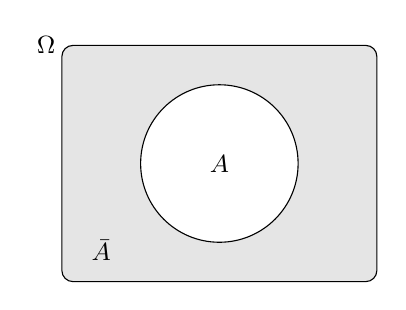
\begin{tikzpicture}[x=10mm,y=10mm,font=\small]
\definecolor{circle area}{gray}{0.9}
\draw[rounded corners, fill=circle area] (0,0) rectangle (4,3) (-.2,3) node {$\Omega$} ;
\node[]  at (.5,.4) {$\bar{A}$};
\draw[fill=white](2,1.5) circle (1) (2,1.5) node {$A$};
\end{tikzpicture}

\caption{La \emph{negazione} di un evento $A$, indicata con $\bar {A}$, è l'evento che si verifica quando non si verifica $A$.}\label{fig:9.1}
\end{minipage}\hfil
\begin{minipage}[t]{.45\textwidth}
\centering% (c) 2013 Claudio Carboncini - claudio.carboncini@gmail.com
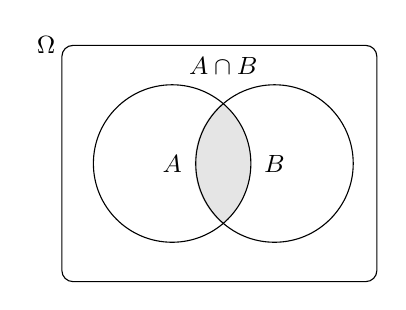
\begin{tikzpicture}[filled/.style={fill=circle area, draw=circle edge, thick},x=10mm,y=10mm,font=\small]
\def\firstcircle{(1.4,1.5) circle (1cm)}
\def\secondcircle{(2.7,1.5) circle (1cm)}

\definecolor{circle edge}{gray}{0.9}
\definecolor{circle area}{gray}{0.9}
    \begin{scope}
        \clip \firstcircle;
        \fill[filled] \secondcircle;
    \end{scope}
    \draw\firstcircle node {$A$};
    \draw \secondcircle node {$B$};
    \node[anchor=south] at (current bounding box.north) {$A \cap B$};
\draw[rounded corners] (0,0) rectangle (4,3) (-.2,3) node {$\Omega$} ;

\end{tikzpicture}

\caption{L'\emph{intersezione} tra gli eventi $A$ e $B$ indicata con $C=A\cap B$ è l'evento che si verifica quando si verificano sia $A$ che $B$.}
\end{minipage}
\vspace{5px}
\begin{minipage}[t]{.45\textwidth}
\centering\input{./lbr/chap09/fig003_uni.pgf}
\caption{L'\emph{unione} tra gli eventi $A$ e $B$ indicata con $C=A\cup B$ è l'evento che si verifica quando si verifica almeno uno dei due eventi.}
\end{minipage}\hfil
\begin{minipage}[t]{.45\textwidth}
\centering% (c) 2013 Claudio Carboncini - claudio.carboncini@gmail.com
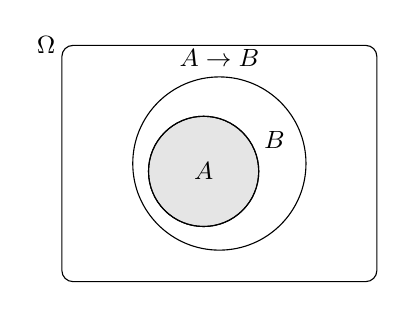
\begin{tikzpicture}[filled/.style={fill=circle area, draw=black, thin},x=10mm,y=10mm,font=\small]
\def\firstcircle{(2,1.5) circle (1.1cm)}
\def\secondcircle{(1.8,1.4) circle (.7cm)}

\definecolor{circle edge}{gray}{0.9}
\definecolor{circle area}{gray}{0.9}
    \begin{scope}
        \clip \firstcircle;
        \fill[filled] \secondcircle;
    \end{scope}
    \draw\firstcircle;
    \node[]  at (2.7,1.8) {$B$}; 
    \draw \secondcircle node {$A$};
    \node[anchor=south] at (current bounding box.north) {$A \to B$};
\draw[rounded corners] (0,0) rectangle (4,3) (-.2,3) node {$\Omega$} ;

\end{tikzpicture}

\caption{L'evento $A$ \emph{implica} l'evento $B$, in simboli $ A \subseteq B$, se ogni volta che si verifica $A$ si verifica anche $B$.}
\end{minipage}
\vspace{5px}
\begin{minipage}[t]{.45\textwidth}
\centering% (c) 2013 Claudio Carboncini - claudio.carboncini@gmail.com
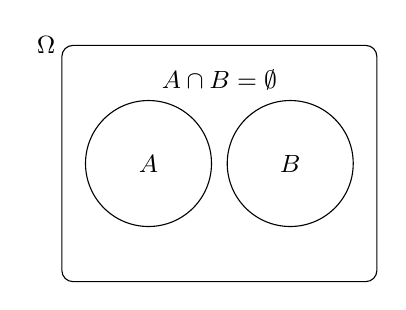
\begin{tikzpicture}[filled/.style={fill=circle area, draw=circle edge, thick},x=10mm,y=10mm,font=\small]
\def\firstcircle{(1.1,1.5) circle (.8cm)}
\def\secondcircle{(2.9,1.5) circle (.8cm)}

\definecolor{circle edge}{gray}{0.8}
\definecolor{circle area}{gray}{0.8}
    \begin{scope}
        \clip \firstcircle;
        \fill[filled] \secondcircle;
    \end{scope}
    \draw\firstcircle node {$A$};
    \draw \secondcircle node {$B$};
    \node[anchor=south] at (current bounding box.north) {$A \cap B=\emptyset$};
\draw[rounded corners] (0,0) rectangle (4,3) (-.2,3) node {$\Omega$} ;

\end{tikzpicture}

\caption{Due eventi $A$ e $B$ si dicono \emph{incompatibili}, se il verificarsi dell'uno esclude il verificarsi dell'altro.}
\end{minipage}\hfil
\begin{minipage}[t]{.45\textwidth}
\centering% (c) 2013 Claudio Carboncini - claudio.carboncini@gmail.com
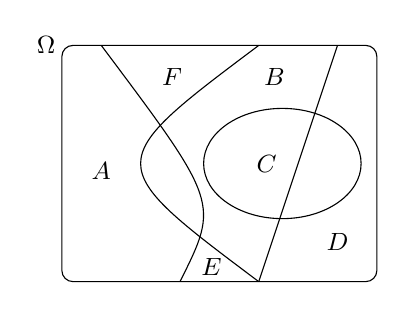
\begin{tikzpicture}[x=10mm,y=10mm,font=\small]
\draw[rounded corners] (0,0) rectangle (4,3) (-.2,3) node {$\Omega$} ;
\draw (.5, 3) .. controls(2,1) .. (1.5, 0);
\node at (.5,1.4) {$A$};
\draw (2.5, 3) .. controls(.5,1.5) .. (2.5, 0);
\node at (2.7,2.6) {$B$};
\draw (2.8,1.5) ellipse (1 and .7);
\node at (2.6,1.5) {$C$};
\draw (3.5,3) -- (2.5,0);
\node at (3.5,.5) {$D$};
\node at (1.9,.18) {$E$};
\node at (1.4,2.6) {$F$};
\end{tikzpicture}

\caption{Due o più eventi si dicono \emph{esaustivi}, se almeno uno di essi si verifica. L'unione di tali eventi coincide con l'insieme $\Omega$.}
\end{minipage}
\vspace{5px}
\begin{minipage}[t]{.90\textwidth}
\centering% (c) 2013 Claudio Carboncini - claudio.carboncini@gmail.com
\begin{tikzpicture}[x=10mm,y=10mm,font=\small]
\draw[rounded corners] (0,0) rectangle (4,3) (-.2,3) node {$\Omega$} ;
%insiemi F ed E
\draw [name path=curva1] (.5, 3) .. controls(2,1) .. (1.5, 0);
\draw [color=white, name path=curva2] (2.5, 3) .. controls(.5,1.5) .. (2.5, 0);
\coordinate [name intersections={of=curva1 and curva2, by={a,b}}];
\draw (a) -- (2.5,3);
\draw (b) -- (2.5,0);
%insiemi B ed D
\draw [name path=elipse1] (2.8,1.5) ellipse (1 and .7);
\draw [color=white, name path=linea1] (3.5,3) -- (2.5,0);
\coordinate [name intersections={of=elipse1 and linea1, by={c,d}}];
\draw (c) -- (3.5,3);
\draw (d) -- (2.5,0);

\node at (.5,1.4) {$A$};
\node at (2.7,2.6) {$B_1$};
\node at (2.6,1.5) {$C$};
\node at (3.5,.5) {$D_1$};
\node at (1.9,.18) {$E$};
\node at (1.4,2.6) {$F$};
\end{tikzpicture}

\caption{Un insieme di eventi formato da eventi tra loro incompatibili ed esaustivi, genera una partizione nello spazio degli eventi.}
\end{minipage}\hfil
\end{figure}

\begin{definizione}
Se $n$ eventi $E_1$, $E_2$, \ldots, $E_n$ sono esaustivi cioè $E_1 \cup E_2 \cup \dots{} \cup E_n=\Omega$ e a due a due tra loro incompatibili $E_1\cap E_2 = E_1 \cap E_3 = \ldots = E_1 \cap E_n = E_2 \cap E_3 = \ldots = E_2 \cap E_4 = \ldots = E_2 \cap E_n = \ldots = E_{n-1}\cap E_n=\emptyset$) diremo che essi formano una \emph{partizione dello spazio degli eventi}. Gli eventi, identificabili da tutti i possibili sottoinsiemi di $\Omega$, sono dati dall'\emph{insieme delle parti} di $\Omega$ indicato con $\wp (\Omega).$
\end{definizione}

Ricordiamo che la cardinalità dell'insieme delle parti cioè il numero degli eventi che si possono formare con gli elementi di $\Omega$ è dato da $\card(\wp(\Omega ))=2^n$, dove $n$ rappresenta il numero degli eventi elementari. Così nel lancio del dado abbiamo $2^6=64$ possibili eventi, considerando anche l'insieme vuoto $\emptyset$ che rappresenta l'evento impossibile e l'insieme $\Omega =\{1$, 2, 3, 4, 5, $6\}$ che rappresenta l'evento certo.

\vspazio\ovalbox{\risolvii \ref{ese:9.1}, \ref{ese:9.2}, \ref{ese:9.3}, \ref{ese:9.4}, \ref{ese:9.5}}

\section{Definizioni di probabilità}

Nel linguaggio comune l'uso del termine probabilità è abbastanza chiaro e uniforme. Si dice che un certo fatto o evento è più o meno probabile a seconda che ci si aspetti che si verifichi più o meno facilmente.

La probabilità è dunque una misura del grado di fiducia associato al verificarsi di un evento e dipende dalle informazioni che si hanno a disposizione al momento di effettuare la valutazione.

Se diciamo che oggi pioverà con probabilità $\np{0,20}=\frac{20}{100}=\frac 1 5$ intendiamo che siamo disposti a scommettere 20 centesimi per avere 1 euro nel caso che piova e perdere i 20 centesimi della posta nel caso che non piova.

\begin{definizione}
La valutazione della probabilità dell'evento $E$ è quel valore $P(E)$ che si ottiene dalla quota $q$ che l'individuo che procede alla valutazione è disposto a pagare per ricevere una vincita $S$ nel caso si verifichi l'evento. Quindi $P(E)=\dfrac q S$.
\end{definizione}

Per ottenere una valutazione coerente, per valutare quanto siamo disposti a perdere/{}vincere nella scommessa, dobbiamo immedesimarci nei due ruoli, quello dello scommettitore e quello del banco. Inoltre le somme che scommettiamo devono essere significative per chi procede alla valutazione.
Nessun individuo coerente scommetterebbe su un evento impossibile una quota maggiore di 0 qualunque sia la vincita e nessun individuo pagherebbe una vincita per il verificarsi di un evento certo.
Da queste considerazioni deduciamo che la misura della probabilità appartiene all'intervallo $[0$, $1]$, essendo $0$ il valore che corrisponde all'evento impossibile e $1$ quello che corrisponde all'evento certo.

\begin{postulato}[sulla probabilità]\label{post:probabilita}
La probabilità di un evento $E$ è un numero reale compreso tra $0$ e $1$: $0\le P(E)\le 1$;

La probabilità dell'evento impossibile è $0$: $P(\emptyset)=0$;

La probabilità dell'evento certo è uguale a $1$: $P(\Omega)=1$.
\end{postulato}

\subsection{La valutazione classica}

La valutazione della probabilità a volte si riconduce a semplici giudizi di equiprobabilità: cioè ogni evento elementare dello spazio degli eventi ha la stessa probabilità. Così nel lancio di un dado, nel gioco della tombola, nel gioco delle carte tutti gli eventi elementari hanno la stessa probabilità. Quindi se $n$ sono gli eventi elementari la probabilità di ciascuno di essi è $\frac 1 n$.

La probabilità di un evento $E$ è data dal rapporto tra il numero $f$ dei casi favorevoli al verificarsi di $E$ e il numero $n$ di tutti i casi possibili, purché ugualmente possibili. In simboli: \[P(E)=\dfrac f n.\]

Mentre nei giochi di sorte si realizzano le condizioni per calcolare tale probabilità (conoscenza a priori dei casi possibili, di quelli favorevoli e condizione di equiprobabilità) esistono altri eventi casuali per i quali è difficile o impossibile calcolare tale probabilità.

\begin{exrig}
\begin{esempio}
Se in un sacchetto ho 3 palline rosse e 2 palline gialle qual è la probabilità che estraendo a caso una pallina questa sia rossa?

La probabilità che si estragga una pallina rossa è $p=\frac 3 5=\np{0,6}=60\text{\%}$, infatti i casi favorevoli al verificarsi dell'evento ``estrarre una pallina rossa'' sono 3, tante quante sono le palline rosse, i casi possibili, tutti ugualmente possibili, sono 5, tante quante palline ci sono nel sacchetto.
\end{esempio}

\begin{esempio}
Da un mazzo di 40 carte napoletane estraiamo una carta. Calcoliamo la probabilità degli eventi:
\begin{itemize*}
\item $A=$ esce una carta di spade;
\item $B=$ esce una carta con il numero 12;
\item $C=$ esce una carta con un numero o una figura;
\item $D=$ esce il sette di denari;
\item $E=$ esce un asso.
\end{itemize*}
I casi possibili sono 40, dato che il mazzo è formato da 40 carte. Anche qui siamo in presenza di eventi elementari equiprobabili, applichiamo ancora lo schema di valutazione classico
\begin{itemize*}
\item L'evento $A$ è casuale, infatti i casi favorevoli sono 10, dato che il mazzo ha 10 carte di spade: $P(A)=\frac{10}{40}=\frac 1 4$;
\item l'evento $B$ è impossibile dato che non esiste una carta col numero 12: $P(B)=0$;
\item l'evento $C$ è certo, infatti i casi favorevoli sono 40, dato che il mazzo ha 12 figure e 28 carte con un numero: $P(C)=1$;
\item c'è un solo sette di denari su 40 carte: $P(D)=\frac 1{40}$;
\item nel mazzo di 40 carte ci sono 4 assi: $P(E)=\frac 4{40}=\frac 1{10}=\np{0,1}=10\%$;
\end{itemize*}
\end{esempio}

\begin{esempio}
Lanciando in aria 3 monete, quale dei seguenti eventi è più probabile?
\begin{itemize*}
\item Ottenere su 3 monete testa;
\item ottenere su 1 moneta testa e su 2 monete croce.
\end{itemize*}
Per rispondere alla domanda occorre calcolare le probabilità dei due eventi. Applichiamo la definizione classica. Dobbiamo calcolare tutti gli eventi possibili e tutti gli eventi favorevoli.
Aiutiamoci con una tabella per elencare tutti i casi.

\begin{center}
\begin{tabular}{ccc}
prima moneta & seconda moneta & terza moneta\\
\boxT & \boxT & \boxT\\
\boxT & \boxT & \boxC\\
\boxT & \boxC & \boxT\\
\boxT & \boxC & \boxC\\
\boxC & \boxT & \boxT\\
\boxC & \boxT & \boxC\\
\boxC & \boxC & \boxT\\
\boxC & \boxC & \boxC\\
\end{tabular}
\end{center}
I casi possibili sono 8. C'è un solo caso favorevole all'evento ``3 volte testa''. La probabilità di questo evento è quindi $p=\frac 1 8=\np{0,125}=\np{12,5}\%$.

I casi favorevoli all'evento ``1 moneta testa e 2 monete croce'' sono CCT, CTC, TCC, quindi 3, allora $p=\frac 3 8=\np{0,375}=\np{37,5}\%$. Possiamo concludere che l'evento più probabile è ottenere 1 testa e 2 croci.
\end{esempio}
\end{exrig}

\subsection{La valutazione sperimentale}

Se si considera una successione di eventi dello stesso tipo e che avvengono in condizioni simili come l'uscita di una determinata faccia in un dado truccato, si indica come frequenza relativa $F(E)$ il rapporto tra il numero $v$ dei casi in cui si è verificato l'evento e il numero totale delle prove $n$, cioè $F(E)=\dfrac v n$.

In una serie di prove ripetute nelle stesse condizioni, la frequenza relativa di un evento tende a stabilizzarsi intorno a un valore ben preciso al crescere del numero delle prove effettuate.
Si assume come valutazione della probabilità dell'evento $E$ il valore intorno al quale tende a stabilizzarsi la frequenza relativa dello stesso evento, all'aumentare del numero delle prove ripetute alle stesse condizioni: $P(E)\approx F(E)=\dfrac v n$.
L'errore che si commette diventa sempre più piccolo al crescere di $n$. La valutazione della probabilità così definita si chiama \emph{valutazione sperimentale}, \emph{statistica}, \emph{a posteriori} o \emph{frequentista}.

Anche l'ambito di applicazione di tale valutazione è limitato in quanto l'ipotesi che sta alla base della definizione è che l'evento a cui si vuole assegnare la probabilità sia pensabile come uno dei possibili risultati di una determinata prova e che tale prova sia ripetibile infinite volte nelle stesse identiche condizioni.
Si fa molto uso di questo schema di valutazione per stime della probabilità in campo economico e sanitario.

\begin{exrig}
\begin{esempio}
In un'azienda alimentare si producono vasetti di marmellata. In uno studio di controllo effettuato su \np{2500} vasetti ne sono stati evidenziati 13 con imperfezioni e non idonei al commercio. Si valuti la probabilità dell'evento $E=$``confezioni non idonee al commercio''.

Se si considera il campione dei vasetti analizzati significativo rispetto alla produzione complessiva delle confezioni prodotte, possiamo considerare la frequenza relativa dell'evento $E$ come misura della probabilità. Quindi $P(E)=F(E)=\frac{13}{\np{2500}}=\np{0,0052}=\np{0,52}\%$.
\end{esempio}

\begin{esempio}
Qual è la probabilità che un certo guidatore faccia un incidente con la macchina? Quanto deve pagare, come premio a una compagnia di assicurazioni, in modo che, se fa un incidente, la compagnia paghi per intero il danno?

Per rispondere a queste domande le compagnie di assicurazioni sono in grado di stimare, sulla base dei numerosissimi incidenti stradali che si verificano ogni anno, qual è la probabilità che un guidatore provochi un incidente d'auto.
\end{esempio}

\begin{esempio}
Un sacchetto contiene 10 palline, alcune bianche, altre nere. Si estrae a caso, senza guardare nel sacchetto un pallina, si guarda il colore e si rimette il sacchetto nella pallina.

Dopo 100 estrazioni abbiamo contato 78 volte la pallina bianca e 22 la pallina nera. Possiamo allora ipotizzare che nel sacchetto ci siano 8 palline bianche e 2 palline nere.
\end{esempio}
\end{exrig}

\subsection{La valutazione soggettiva}

La valutazione soggettiva della probabilità è la definizione che abbiamo dato all'inizio del capitolo: la probabilità dell'evento $A$ è quel valore $p$ che l'individuo che procede alla valutazione è disposto a pagare per ricevere una vincita unitaria. Se un individuo valuta pari $\frac 1 4=25\%$ la probabilità di un certo evento $E$ vuol dire che è disposto a pagare $25$ euro a un ipotetico banco per riceverne $100$ nel caso che $E$ si verifichi. Naturalmente la scommessa va accettata anche come banco che deve essere disposto a scommettere il $75\%=1-p$ sul fatto che $E$ non si verifichi: $P(E)=\frac q S$ con $ q=25 $ e $S=100$.

\subsubsection*{Le scommesse}

La definizione soggettiva si applica anche alle scommesse. Supponiamo di scommettere sul verificarsi di un evento $E$ a cui attribuiamo probabilità $p$. Stabiliamo inoltre di giocare e quindi perdere $q$ euro nel caso l'evento non si verifichi e di guadagnare $g$ euro nel caso l'evento si verifichi. In genere le scommesse si indicano in questo modo: si mette in rapporto il guadagno con la perdita $\frac g q$ o anche $g:q$ che si legge $g$ a $q$. In questo caso $q$ e $g$ si chiamano le \emph{poste} o le \emph{messe} del gioco.

%si mette in rapporto la perdita con il guadagno $\frac q g$ o anche $q:g$ che si legge $q$ a $g$. In questo caso $q$ e $g$ si chiamano le \emph{poste} o le \emph{messe} del gioco.

Che relazione c'è tra questo rapporto e la probabilità?

Se in un grande numero $n$ di scommesse così congegnate vincessimo la somma $g$ per $np$ di volte e perdessimo la somma $q$ per $n(1-p)$ volte, affinché il gioco risulti \emph{equo} dovremmo avere $np\cdot g-nq\cdot (1-p)=0 \:\Rightarrow\: n(p\cdot g-q\cdot (1-p))=0$ e visto che $n\neq 0$ si può dividere per $n$ ottenendo $p\cdot g-q\cdot (1-p)=0$. Isoliamo $p$ nell'uguaglianza:
\begin{equation*}
p\cdot g-q\cdot (1-p)=0 \:\Rightarrow\: p\cdot g-q+q\cdot p=0\:\Rightarrow\: p\cdot (g+q)=q \:\Rightarrow\: p=\frac q{g+q}.
\end{equation*}
La relazione è dunque questa: la probabilità di una scommessa $g:q$ è data dalla perdita $q$ al numeratore e al denominatore la somma complessiva che si incassa data dal guadagno più quello che si è scommesso.

\begin{exrig}
\begin{esempio}
Supponiamo che la vincita ai mondiali di calcio dell'Italia sia data $12:5$, cioè 12 a 5, dai bookmaker inglesi. Quale probabilità assegnano gli allibratori alla vincita dell'Italia?

Significa che scommettendo 5 euro sulla vincita dell'Italia ne possiamo vincere 12 nel caso che l'evento si verifichi.

Quindi la probabilità della vincita dell'Italia sarà:
$P(E)=\frac 5{5+12}=\frac 5{17}=\np{0,294}=\np{29,4}\%$
\end{esempio}

\begin{esempio}
Leggo sul sito del Corriere della Sera, che per la partita Real Madrid-Barcellona, che si giocherà questa sera, la vittoria del Real Madrid viene data \np{2,60} a 1.

Significa che scommettendo 1 euro possiamo vincerne \np{2,60}: la vittoria del Real Madrid è stata quindi stimata dal giornale $p=\frac 1{\np{2,60}}=\frac{100}{260}=\np{0,38}\ldots$ circa 38\%.
\end{esempio}
\end{exrig}
\ovalbox{\risolvii \ref{ese:9.6}, \ref{ese:9.7}, \ref{ese:9.8}, \ref{ese:9.9}, \ref{ese:9.10}, \ref{ese:9.11}, \ref{ese:9.12}, \ref{ese:9.13}, \ref{ese:9.14}, \ref{ese:9.15}, \ref{ese:9.16},}

\vspazio\ovalbox{\ref{ese:9.17}, \ref{ese:9.18}, \ref{ese:9.19}, \ref{ese:9.20}, \ref{ese:9.21}, \ref{ese:9.22}, \ref{ese:9.23}, \ref{ese:9.24}, \ref{ese:9.25}, \ref{ese:9.26}, \ref{ese:9.27}}

\section{Probabilità dell'unione di due eventi}

La misura della probabilità si può applicare a tutti gli eventi individuati dall'insieme delle parti degli eventi elementari $\wp(\Omega)$. Qualsiasi evento si può definire come sottoinsieme dell'insieme elementare (elencando gli eventi elementari che ne fanno parte) oppure enunciando una proposizione vera nel caso in cui l'evento si verifichi. Possiamo quindi poter esprimere la probabilità su eventi composti da due o più eventi di $\wp(\Omega)$ attraverso le operazioni di unione e intersezione tra insiemi che corrispondono alle operazioni di disgiunzione inclusiva e di congiunzione nelle proposizioni.

Per la probabilità dell'evento unione di due eventi occorre distinguere tra eventi tra loro \emph{incompatibili} ed eventi tra loro \emph{compatibili}.

\subsection[Unione di due eventi tra loro incompatibili]{Unione di due eventi tra loro incompatibili}

\begin{definizione}
Due eventi $A$ e $B$ si dicono \emph{incompatibili} quando non si possono verificare contemporaneamente, cioè quando $A\cap B=\emptyset$.
\end{definizione}

\begin{definizione}
Due eventi $A$ e $B$ si dicono \emph{compatibili} quando si possono verificare contemporaneamente, cioè quando $A\cap B\neq \emptyset$.
\end{definizione}
\pagebreak
\begin{exrig}
\begin{esempio}
Nel lancio di un dado regolare calcolare la probabilità dell'uscita del numero 3 o di un numero pari.

I due eventi $A=$``uscita del numero 3'' e $B=$``uscita di un numero pari'' sono eventi incompatibili.

Ci sono due modi per calcolare la probabilità dell'evento unione.
\paragraph{Modo I}: Secondo la valutazione classica la probabilità che esca il $3$ o un numero pari è uguale a $\frac 4 6$: infatti i casi favorevoli sono 4 (le facce 3, 2, 4 e 6) su un totale di $6$ casi possibili.
\paragraph{Modo II}: Calcoliamo la probabilità dell'unione dei due eventi considerando le proprietà dei singoli eventi. Dato che i due eventi sono incompatibili, cioè: $A\cap B=\emptyset $: abbiamo $P(A\cup B)=\frac 1 6+\frac 3 6=\frac 4 6$.
\begin{center}
 % (c) 2013 Claudio Carboncini - claudio.carboncini@gmail.com
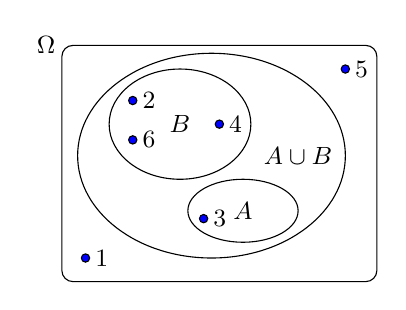
\begin{tikzpicture}[x=10mm,y=10mm,font=\small]
\def\insieme_unione{(1.9,1.6) ellipse (1.7 and 1.3)}
\def\insiemeB{(1.5,2) ellipse (.9 and .7)}
\def\insiemeA{(2.3,.9) ellipse (.7 and .4)}
\draw[rounded corners] (0,0) rectangle (4,3) (-.2,3) node {$\Omega$} ;
\draw\insieme_unione;
\draw\insiemeB node {$B$};
\draw\insiemeA node {$A$};
\draw[fill=blue] (.9,2.3)circle (1.5pt) node[right]{$2$};
\draw[fill=blue] (.9,1.8)circle (1.5pt) node[right]{$6$};
\draw[fill=blue] (2,2)circle (1.5pt) node[right]{$4$};
\draw[fill=blue] (1.8,.8)circle (1.5pt) node[right]{$3$};
\draw[fill=blue] (.3,.3)circle (1.5pt) node[right]{$1$};
\draw[fill=blue] (3.6,2.7)circle (1.5pt) node[right]{$5$};
\node at (3,1.6) {$A \cup B$};
\end{tikzpicture}

\end{center}
\end{esempio}
\end{exrig}

Possiamo quindi affermare che dati due eventi incompatibili cioè tali che $A\cap B=\emptyset$ la probabilità dell'evento unione è dato dalla uguaglianza: $P(A\cup B)=P(A)+P(B)$.

Può essere utile per avere un'idea intuitiva di questa uguaglianza pensare alla probabilità come una massa unitaria distribuita sugli eventi. Se voglio la probabilità di $A\cup B$, considero la massa presente su $A$ che addiziono a quella presente su $B$ (in analogia al caso dell'unione di insiemi disgiunti).

\subsection{Unione di due eventi tra loro compatibili}

\begin{exrig}
\begin{esempio}
Consideriamo il lancio di un dado regolare, vogliamo trovare la probabilità dell'uscita di un numero maggiore di 2 o di un numero dispari.

Gli eventi $A=$``uscita di un numero maggiore di 2'' e $B=$``uscita di un numero dispari'' sono compatibili in quanto le facce 5 e 3 appartengono sia all'evento $A$ che all'evento $B$.
\begin{center}
 % (c) 2013 Claudio Carboncini - claudio.carboncini@gmail.com
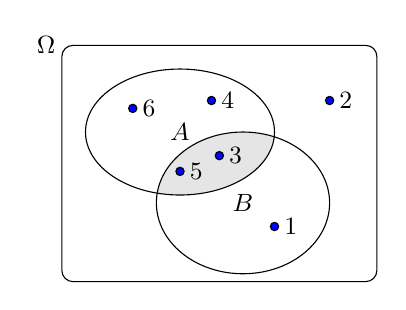
\begin{tikzpicture}[x=10mm,y=10mm,font=\small]

\def\insiemeA{(1.5,1.9) ellipse (1.2 and .8)}
\def\insiemeB{(2.3,1) ellipse (1.1 and .9)}
    \begin{scope}
        \clip \insiemeA;
        \fill[color=gray!20!] \insiemeB;
    \end{scope}
\draw[rounded corners] (0,0) rectangle (4,3) (-.2,3) node {$\Omega$} ;
\draw\insiemeB node {$B$};
\draw\insiemeA node {$A$};
\draw[fill=blue] (.9,2.2)circle (1.5pt) node[right]{$6$};
\draw[fill=blue] (3.4,2.3)circle (1.5pt) node[right]{$2$};
\draw[fill=blue] (1.9,2.3)circle (1.5pt) node[right]{$4$};
\draw[fill=blue] (2.7,.7)circle (1.5pt) node[right]{$1$};
\draw[fill=blue] (2,1.6)circle (1.5pt) node[right]{$3$};
\draw[fill=blue] (1.5,1.4)circle (1.5pt) node[right]{$5$};

\end{tikzpicture}

\end{center}
\paragraph{Modo I}: La probabilità che esca un numero maggiore di $2$ o un numero dispari è uguale a $\frac 5 6$: infatti i casi favorevoli sono 5 (le facce 1, 3, 4, 5 e 6) su un totale di $6$ casi possibili.
\paragraph{Modo II}: Calcoliamo la probabilità dell'unione dei due eventi considerando le proprietà dei singoli eventi. In questo caso non possiamo sommare come nei casi precedenti le probabilità dei singoli eventi. Infatti $P(A)+P(B)=\frac 4 6+\frac 3 6=\frac 7 6$ che contraddice l'assioma della probabilità. Occorre togliere la probabilità dell'intersezione tra $A$ e $B$ contata due volte, una volta per $A$ e una per $B$, che è uguale a $\frac 2 6$: due casi favorevoli (le facce 3 e 5) su sei casi possibili: \[P(A\cup B)=P(A)+P(B)-P(A\cap B)=\frac 4 6+\frac 3 6-\frac 2 6=\frac 5 6.\]
\end{esempio}

\begin{esempio}
Calcolare la probabilità che estraendo a caso un numero della tombola esso contenga la cifra 5 oppure sia multiplo di 5.

La prima domanda da farsi è se i due eventi sono compatibili o incompatibili. Poiché esistono numeri della tombola che contengono la cifra 5 e che sono anche multipli di 5 (per esempio 15, 50, \ldots) i due eventi sono compatibili. Di conseguenza bisogna applicare la regola $P(A\cup B)=P(A)+P(B)-P(A\cap B)$.
\begin{itemize*}
\item $A=$``estrarre un numero che contiene la cifra 5''. Questi numeri sono: 5, 15, 25, 35, 45, 50, 51, 52, \ldots, 59, 65, 75, 85, in tutto 18 ne segue che: $p(A)=\frac{18}{90}$;
\item $B=$``estrarre un numero multiplo di 5''. I multipli di 5 sono 5, 10, 15, 20, \ldots{} due per ogni decina, quindi 18 in tutto, ne segue che: $p(B)=\frac{18}{90}$;
\item $A\cap B=$``estrarre un cifra che contiene 5 ed è multiplo di 5''. Questi numeri sono 5, 15, 25, 35, 45, 50, 55, 65, 75, 85 in tutto sono 10 quindi: $p(A\cap B)=\frac{10}{90}$.
\end{itemize*}
Applichiamo la regola della probabilità utilizzata nel modo II del precedente esempio quindi:

$A\cup B=$``estrarre un numero che contenga la cifra 5 oppure sia multiplo di 5''. \[P(A\cup B)=P(A)+P(B)-P(A\cap B)=\frac{18}{90}+\frac{18}{90}-\frac{10}{90}=\frac{26}{90}\simeq \np{0,29}= 29\%. \]
\end{esempio}
\end{exrig}

Dagli esempi svolti possiamo enunciare il seguente teorema:

\begin{teorema}[delle probabilità totali]
Dati due eventi $A$ e $B$, entrambi appartenenti allo stesso spazio degli eventi, la probabilità dell'unione degli eventi è uguale alla somma delle probabilità dei singoli eventi meno la probabilità della loro intersezione.
In simboli: \[P(A\cup B)=P(A)+P(B)-P(A\cap B).\]
\end{teorema}

Se pensiamo alla probabilità come una massa unitaria distribuita sugli eventi, per calcolare la probabilità di $A\cup B$, considero la massa presente su $A$ che addiziono a quella presente su $B$ a cui devo togliere la massa presente su $A\cap B$ che è stata contata due volte.

\osservazione Il teorema delle proprietà totali vale anche nel caso degli eventi incompatibili in quanto in questo caso la probabilità dell'intersezione dei due eventi $P(A\cap B)=\emptyset$ e l'uguaglianza diventa $P(A\cup B)=P(A)+P(B)$.

\vspazio\ovalbox{\risolvii \ref{ese:9.6}, \ref{ese:9.7}, \ref{ese:9.28}, \ref{ese:9.29}, \ref{ese:9.30}, \ref{ese:9.31}, \ref{ese:9.32}, \ref{ese:9.33}, \ref{ese:9.34}, \ref{ese:9.35}, \ref{ese:9.36},}

\ovalbox{\ref{ese:9.37} \ref{ese:9.38}}

\section{Probabilità dell'evento complementare }

\begin{definizione}
Dato un evento $A$, si definisce \emph{evento complementare} di $A$, indicato con $\overline A$, l'evento che si verifica quando non si verifica $A$.
\end{definizione}

\begin{teorema}[dell'evento complementare]
Dato un evento $E$, la probabilità dell'evento complementare $\overline E$ è data da $1$ meno la probabilità dell'evento $E$. In simboli: \[ P(\overline E)=1-P(E). \]
\end{teorema}
\begin{proof} Per il postulato~\ref{post:probabilita} introdotto a pagina~\pageref{post:probabilita}: \[ P(\overline E\cup E)=P(\Omega)=1; \]
per il teorema delle probabilità totali essendo i due eventi incompatibili: \[ P(\overline E\cup E)=P(\overline E)+P(E); \]
e per la proprietà transitiva dell'uguaglianza: \[ P(\overline E)+P(E)=1 \quad\Rightarrow\quad P(\overline E)=1-P(E). \]
\end{proof}

Se pensiamo all'analogia della una massa unitaria distribuita sugli eventi, la probabilità dell'evento $\overline E$ sarà data dalla massa unitaria meno la probabilità di $E$.

\begin{exrig}
\begin{esempio}
Nel lancio di due dadi regolari determina la probabilità che la somma delle facce non sia uguale a 5.

Consideriamo la probabilità che in un lancio di due dadi si abbia un punteggio uguale a 5. I casi possibili sono 36 (ogni faccia del primo dado si può associare con ognuna delle 6 facce del secondo dado), mentre i casi favorevoli all'evento sono 4, precisamente $(1$, $4)$, $(4$, $1)$, $(2$, $3)$ e $(3$, $2)$. Quindi $P(E)=\frac 4{36}=\frac 1 9$.

Per conoscere la probabilità dell'evento complementare cioè la probabilità che la somma delle due facce del dado non sia uguale a 5, risulterebbe piuttosto laborioso trovare tutti i casi in cui la somma delle due facce sia uguale a 2, 3, 4, 6, 7, 8, 9, 10, 11 e 12, si può invece applicare la regola $P(\overline E)=1-P(E)$ cioè nel nostro caso $P(\overline E)=1-P(E)=1-\frac 1 9=\frac 8 9$.
\end{esempio}
\end{exrig}

\osservazione L'uguaglianza sulla probabilità dell'evento complementare può risultare molto utile per risolvere alcuni problemi. A volte è più facile, o indispensabile, calcolare la probabilità dell'evento complementare che calcolare direttamente la probabilità dell'evento.

\vspazio\ovalbox{\risolvii \ref{ese:9.39}, \ref{ese:9.40}, \ref{ese:9.41}, \ref{ese:9.42}, \ref{ese:9.43}, \ref{ese:9.44}, \ref{ese:9.45}, \ref{ese:9.46}}

\section{La probabilità dell'evento intersezione di due eventi}

Dati due eventi $A$, $B\in \wp(\Omega)$ ci proponiamo di calcolare la probabilità dell'evento intersezione cioè $P(A\cap B)$ partendo dalla probabilità degli eventi componenti $P(A)$ e $P(B)$. Si tratta quindi di stimare con quale probabilità i due eventi avvengono congiuntamente. Occorre innanzitutto verificare che i due eventi non siano incompatibili in quanto in questo caso l'evento intersezione è impossibile.

Per la probabilità dell'intersezione di due eventi occorre distinguere tra eventi tra loro \emph{indipendenti} e eventi tra loro \emph{dipendenti}.

\subsection{Intersezione di due eventi tra loro indipendenti}

\begin{definizione}
Due eventi $A$ e $B$ si dicono \emph{indipendenti} se il verificarsi di $A$ non cambia la probabilità del verificarsi di $B$, si dicono invece \emph{dipendenti} se il verificarsi di $A$ cambia la probabilità di $B$ rispetto a quella valutata per $B$ prima del verificarsi di $A$.
\end{definizione}

%\newpage

\begin{exrig}
\begin{esempio}
Determinare la probabilità che lanciando una moneta e un dado regolari esca testa e un numero maggiore di 4.
\begin{itemize}
\item $A=$``uscita di Testa nel lancio di una moneta'' $\Rightarrow\: P(A)=\frac 1 2$;
\item $B=$``uscita di un numero maggiore di 4 nel lancio di un dado'' $\Rightarrow\: P(B)=\frac 2 6$;
\item $(A\cap B)$=``uscita di testa e di un numero maggiore di 4 nel lancio di una moneta e di un dado''.
\end{itemize}
Vediamo come determinare $P(A\cap B)$.
I due eventi $A$ e $B$ non si influenzano in quanto l'uscita di testa non modifica la probabilità dell'uscita di 4 nel lancio del dado.

Notiamo subito una situazione diversa rispetto a quella precedente dell'unione di due eventi. Nel caso precedente, lo spazio degli eventi era lo stesso per l'evento $A$, per l'evento $B$ e per l'evento unione $(A\cup B)$.
Ora invece per l'evento $A$ l'insieme degli eventi elementari è $\Omega_1=\{T$, $C\}$, per l'evento $B$ invece, l'insieme degli eventi elementari è $\Omega_2=\{1$, 2, 3, 4, 5, $6\}$. L'evento $(A\cap B)$ ha il seguente insieme degli eventi elementari: \[\Omega=\{(T;1)\text{, }(T;2)\text{, }(T;3)\text{, }(T;4)\text{, }(T;5)\text{, }(T;6)\text{, }(C;1)\text{, }(C;2)\text{, }(C;3)\text{, }(C;4)\text{, }(C;5)\text{, }(C;6)\}. \]

Lo spazio degli eventi elementari dell'intersezione è dato dal prodotto cartesiano dello spazio elementare di $A$ moltiplicato per quello di $B$. Si può calcolare la probabilità in due modi:
\paragraph{Modo I}: Si indicano i casi favorevoli e i casi possibili rispetto all'evento intersezione: i casi favorevoli all'evento sono due: $(A\cap B)=\{(T;5)\text{, }(T;6)\}$, i casi possibili sono dodici: \[\Omega=\{(T;1)\text{, }(T;2)\text{, }(T;3)\text{, }(T;4)\text{, }(T;5)\text{, }(T;6)\text{, }(C;1)\text{, }(C;2)\text{, }(C;3)\text{, }(C;4)\text{, }(C;5)\text{, }(C;6)\} \] la probabilità dell'evento intersezione è: $P(A\cap B)=\frac 2{12}=\frac 1 6$.

\begin{center}
 % (c) 2013 Claudio Carboncini - claudio.carboncini@gmail.com
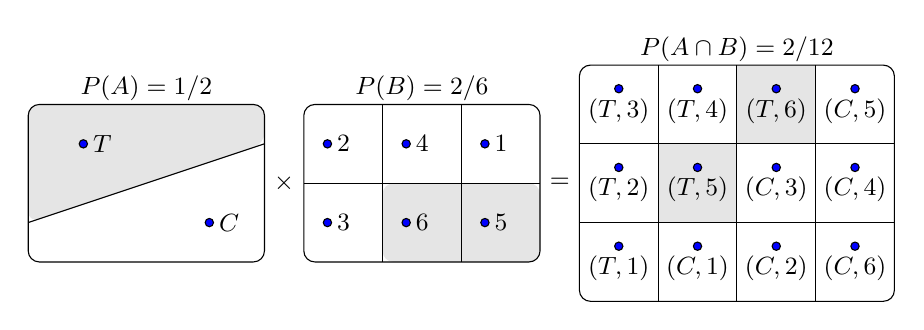
\begin{tikzpicture}[x=10mm,y=10mm,font=\small]

\def\rettangolo{-- ++(3,0) -- ++(0,2) -- ++(-3,0) -- cycle}
\def\insieme_int{-- ++(4,0) -- ++(0,3) -- ++(-4,0) -- cycle}
 %insieme1
\fill[rounded corners, color=gray!20!] (0,.5) -- (0,2) -- (3,2) -- (3,1.5) -- cycle;
\draw[rounded corners] (0,0) \rettangolo;
\node at (1.5,2.2) {$P(A)=1/2$};
\draw (0,.5) -- (3,1.5);
\draw[fill=blue] (.7,1.5) circle (1.5pt) node[right] {$T$};
\draw[fill=blue] (2.3,.5) circle (1.5pt) node[right] {$C$};
%insieme 2
\fill[rounded corners, color=gray!20!] (4.5,0) -- (6.5,0) -- (6.5,1) -- (4.5,1) -- cycle;
\draw[rounded corners] (3.5,0) \rettangolo;
\draw (3.5,1) -- (6.5,1);
\foreach \x in {4.5,5.5}{
\draw (\x,0)--(\x,2);
\draw (\x,0)--(\x,2);}
\foreach \x in {3.8,4.8,5.8}
   \foreach \y in {0.5,1.5}
   { \draw[fill=blue] (\x,\y) circle (1.5pt);}
\draw node[right] at (3.8,1.5) {$2$};
\draw node[right] at (4.8,1.5) {$4$};
\draw node[right] at (5.8,1.5) {$1$};

\draw node[right] at (3.8,0.5) {$3$};
\draw node[right] at (4.8,0.5) {$6$};
\draw node[right] at (5.8,0.5) {$5$};
\node at (5,2.2) {$P(B)=2/6$};
\node at (3.25,1) {$\times$};
%insieme risultato
\fill[color=gray!20!] (8,.5) -- (8,1.5) -- (9,1.5) -- (9,.5) -- cycle;
\fill[color=gray!20!] (9,1.5) -- (9,2.5) -- (10,2.5) -- (10,1.5) -- cycle;
\draw[rounded corners] (7,-.5) \insieme_int;
\node at (9,2.7) {$P(A \cap B )=2/12$};
\node at (6.75,1) {$=$};
\foreach \x in {8,9,10}{
\draw (\x,-.5)--(\x,2.5);
\draw (\x,-.5)--(\x,2.5);
\draw (\x,-.5)--(\x,2.5);}
\foreach \y in {.5,1.5}{
\draw (7,\y)--(11,\y);
\draw (7,\y)--(11,\y);}

\foreach \x in {7.5,8.5,9.5,10.5}
   \foreach \y in {0.2,1.2,2.2}
   { \draw[fill=blue] (\x,\y) circle (1.5pt);}
\draw node[below] at (7.5,0.2) {$(T,1)$};
\draw node[below] at (8.5,0.2) {$(C,1)$};
\draw node[below] at (9.5,0.2) {$(C,2)$};
\draw node[below] at (10.5,0.2) {$(C,6)$};

\draw node[below] at (7.5,1.2) {$(T,2)$};
\draw node[below] at (8.5,1.2) {$(T,5)$};
\draw node[below] at (9.5,1.2) {$(C,3)$};
\draw node[below] at (10.5,1.2) {$(C,4)$};

\draw node[below] at (7.5,2.2) {$(T,3)$};
\draw node[below] at (8.5,2.2) {$(T,4)$};
\draw node[below] at (9.5,2.2) {$(T,6)$};
\draw node[below] at (10.5,2.2) {$(C,5)$};

\end{tikzpicture}

\end{center}

\paragraph{Modo II}: Dato che i due eventi non si influenzano, supponiamo di procedere con due scelte successive: prima il lancio della moneta con probabilità pari a $\frac 1 2$ e poi il lancio del dado con probabilità pari a $\frac 2 6$. Se si verifica il primo evento la probabilità si riduce da 1 a $\frac 1 2$ a cui devo applicare la probabilità che si verifichi il secondo evento pari a $\frac 2 6$, moltiplicando le probabilità dei singoli eventi.
\begin{itemize*}
\item $A=$``uscita di Testa nel lancio di una moneta'' $\Rightarrow\: P(A)=\frac 1 2$;
\item $B=$``uscita di un numero maggiore di 4 nel lancio di un dado'' $\Rightarrow\: P(B)=\frac 2 6$;
\item $(A\cap B)$=``uscita di testa e di un numero maggiore di 4 nel lancio di una moneta e di un dado'' $\Rightarrow\: P(A\cap B)=P(A)\cdot P(B)=\frac 1 2\cdot \frac 2 6=\frac 2{12}$.
\end{itemize*}
\end{esempio}
\end{exrig}

Generalizziamo: dati due eventi aleatori $A$ e $B$ tra loro indipendenti la probabilità dell'evento intersezione tra $A$ e $B$ è data dalla probabilità di $A$ moltiplicata per la probabilità di $B$: \[P(A\cap B)=P(A)\cdot P(B).\]\label{reg:probabilita_intersezione_eventi_indipendenti}

\subsubsection*{Diagrammi ad albero}

Una rappresentazione grafica che può risultare utile nello studio della probabilità dell'evento intersezione detto anche studio delle \emph{probabilità composte} è il diagramma ad albero. Le linee dell'albero si dicono \emph{rami}, mentre i punti da cui partono e arrivano i rami si dicono \emph{nodi}, il nodo iniziale si chiama \emph{radice}.

La costruzione di un diagramma ad albero nel caso delle probabilità composte consente di eseguire un'analisi completa di tutti i possibili esiti di una prova. Ogni percorso dell'albero che va dalla radice al nodo terminale indica una sequenza di eventi congiunti, incompatibile con qualsiasi altro percorso dell'albero. La probabilità di ogni singolo evento si indica sui rami e moltiplicando le probabilità che si incontrano nel percorso si ottiene la probabilità della congiunzione degli eventi che formano il percorso. Dato che ogni percorso che va dalla radice al nodo terminale individua eventi incompatibili, se vogliamo trovare l'unione di due o più percorsi possiamo semplicemente sommarli.
L'esempio precedente può essere schematizzato in questo modo:
\begin{center}
 % (c) 2012 Dimitrios Vrettos - d.vrettos@gmail.com
\begin{tikzpicture}[x=10mm,y=10mm,font=\small]
\node [circle, draw] (a) {$\bullet$};
\node [circle, draw, fill=orange!20!] (t) [above right=of a] {$T$};
\node [circle, draw] (c) [below right=of a] {$C$};
\node [rectangle, draw] (d1) at(45:5.5) {$1$};
\node [right=.1 of d1]{$P(T \cap 1)=1/12$};
\node [rectangle, draw] (d2) [below =.2 of d1] {$2$};
\node [right=.1 of d2]{$P(T \cap 2)=1/12$};
\node [rectangle, draw] (d3) [below =.2 of d2] {$3$};
\node [right=.1 of d3]{$P(T \cap 3)=1/12$};
\node [rectangle, draw] (d4) [below =.2 of d3] {$4$};
\node [right=.1 of d4]{$P(T \cap 4)=1/12$};
\node [rectangle, draw, fill=orange!20!] (d5) [below =.2 of d4] {$5$};
\node [right=.1 of d5] (ad1){$P(T \cap 5)=1/12$};
\node [rectangle, draw, fill=orange!20!] (d6) [below =.2 of d5] {$6$};
\node [right=.1 of d6] (ad2){$P(T \cap 6)=1/12$};
\draw (6.7,.55) -- (7.2,.55) -- (7.2,1.2) -- (6.7,1.2);
\node at (7.4,.9) {$+$};
\node [rectangle, draw] (d11) [below =.2 of d6] {$1$};
\node [right=.1 of d11]{$P(C \cap 1)=1/12$};
\node [rectangle, draw] (d22) [below =.2 of d11] {$2$};
\node [right=.1 of d22]{$P(C \cap 2)=1/12$};
\node [rectangle, draw] (d33) [below =.2 of d22] {$3$};
\node [right=.1 of d33]{$P(C \cap 3)=1/12$};
\node [rectangle, draw] (d44) [below =.2 of d33] {$4$};
\node [right=.1 of d44]{$P(C \cap 4)=1/12$};
\node [rectangle, draw] (d55) [below =.2 of d44] {$5$};
\node [right=.1 of d55]{$P(C \cap 5)=1/12$};
\node [rectangle, draw] (d66) [below =.2 of d55] {$6$};
\node [right=.1 of d66]{$P(C \cap 6)=1/12$};

\draw[ultra thick,color=Maroon] (a) -- (t) node[midway,sloped,above] {$1/2$};
\draw (a) -- (c)node[midway,sloped,above] {$1/2$};
\draw (t) -- (d1)node[midway,sloped] {$1/6$};
\draw (t) -- (d2)node[midway,sloped] {$1/6$};
\draw (t) -- (d3)node[midway,sloped] {$1/6$};
\draw (t) -- (d4)node[midway,sloped] {$1/6$};
\draw[thick,color=Maroon] (t) -- (d5)node[midway,sloped] {$1/6$};
\draw[thick,color=Maroon] (t) -- (d6)node[midway,sloped] {$1/6$};
\draw (c) -- (d11)node[midway,sloped] {$1/6$};
\draw (c) -- (d22)node[midway,sloped] {$1/6$};
\draw (c) -- (d33)node[midway,sloped] {$1/6$};
\draw (c) -- (d44)node[midway,sloped] {$1/6$};
\draw (c) -- (d55)node[midway,sloped] {$1/6$};
\draw (c) -- (d66)node[midway,sloped] {$1/6$};

\end{tikzpicture}

\end{center}
L'albero può essere semplificato considerando gli eventi coinvolti e i loro complementari.

\begin{exrig}
\begin{esempio}
In un'urna abbiamo tre palline bianche e due nere. Facciamo due estrazioni rimettendo dopo la prima estrazione la pallina nell'urna. Vogliamo calcolare la probabilità dell'uscita di una pallina nera nelle due estrazioni.
\begin{itemize*}
\item $B_{1}=$``nella prima estrazione pallina bianca'' $\Rightarrow\: P(B_1)=\frac 3 5$;
\item $B_{2}=$``nella seconda estrazione pallina bianca'' $\Rightarrow\: P(B_2)=\frac 3 5$ in quanto la pallina si rimette nell'urna;
\item $N_{1}=$``nella prima estrazione pallina nera'' $\Rightarrow\: P(N_1)=\frac 2 5$;
\item $N_{2}=$``nella seconda estrazione pallina nera'' $\Rightarrow\: P(N_2)=\frac 2 5$.
\end{itemize*}
Il problema è sempre lo stesso: calcolare una probabilità su un insieme intersezione partendo dalle probabilità degli eventi componenti. Devo moltiplicare la probabilità di avere nera nella prima estrazione $P(N_1)=\frac 2 5$ con la probabilità di avere nera nella seconda estrazione $P(N_2)=\frac 2 5$ in quanto, l'uscita della prima pallina nera, evento considerato ora come avvenuto, non influenza la probabilità di avere nera alla seconda estrazione in quanto la pallina estratta viene rimessa nell'urna. Quindi: $P(N_1\cap N_2)=\frac 2 5\cdot \frac 2 5=\frac 4{25}$ in quanto i due eventi sono indipendenti.
\begin{center}
 % (c) 2013 Claudio Carboncini - claudio.carboncini@gmail.com
\begin{tikzpicture}[x=10mm,y=10mm,font=\small]

\filldraw[fill=gray!20!, draw=black]
(.7,-1)--(.7,1)--(.9,1)--(.9,-.8)--(3,-.8)--(3,1)--(3.2,1)--(3.2,-1)-- cycle;
\filldraw[fill=black, draw=black]  (1.2,.5) circle (4pt);
\filldraw[fill=black, draw=black]  (2.5,-.3) circle (4pt);
\filldraw[fill=white, draw=black]  (1.4,0) circle (4pt);
\filldraw[fill=white, draw=black]  (2.4,.4) circle (4pt);
\filldraw[fill=white, draw=black]  (1.9,-.5) circle (4pt);

\node [circle, draw] (a) at (5,0) {$\bullet$};
\node [circle, draw] (b1) [above right=of a] {$B_1$};
\node [circle, draw, fill=orange!20!] (n1) [below right=of a] {$N_1$};
\node [circle, draw] (b2) at(15:9) {$B_2$};
\node [right=.1 of b2] {$P(B_1 \cap B_2)=9/25$};
\node [circle, draw] (n2) [below =.7 of b2] {$N_2$};
\node [right=.1 of n2] {$P(B_1 \cap N_2)=6/25$};
\node [circle, draw] (b3) [below =.7 of n2] {$B_2$};
\node [right=.1 of b3] {$P(N_1 \cap B_2)=6/25$};
\node [circle, draw, fill=orange!20!] (n3) [below =.7 of b3] {$N_2$};
\node [right=.1 of n3] {$P(N_1 \cap N_2)=4/25$};
\draw (a) -- (b1)node[midway,sloped,above] {$3/5$};
\draw[ultra thick,color=Maroon] (a) -- (n1) node[midway,sloped,above] {$2/5$};
\draw (b1) -- (b2)node[midway,sloped,above] {$3/5$};
\draw (b1) -- (n2)node[midway,sloped,above] {$2/5$};
\draw (n1) -- (b3)node[midway,sloped,above] {$3/5$};
\draw[thick,color=Maroon] (n1) -- (n3) node[midway,sloped,above] {$2/5$};

\end{tikzpicture}

\end{center}

Le domande che posso fare su questo esperimento sono relative allo spazio degli eventi $\wp(\Omega).$ ove $\Omega =\{(B_1;B_2)$, $(B_1;N_2)$, $(N_1;B_2)$, $(N_1;N_2)\}$ sono del tipo ``Qual è la probabilità che nelle due estrazioni escano palline di diverso colore'', ``Qual è la probabilità che la prima pallina sia bianca'', ecc.
\end{esempio}
\end{exrig}

\subsubsection*{Il problema del Cavalier de Méré}

Il Cavalier de Méré pose al grande matematico francese Blaise Pascal nel 1654 il seguente problema.
\begin{problema}
Perché scommettendo alla pari sull'evento $A=$``ottenere almeno una volta un 6 in 4 lanci di un dado'' ho accumulato una fortuna, mentre rischio la rovina scommettendo alla pari sull'evento $B=$``ottenere almeno una coppia di 6 in 24 lanci di due dadi''.
\end{problema}
Scommettere alla pari, 1:1, significa assegnare alla probabilità degli eventi $A$ e $B$ il valore pari a $\frac 1 2$.
Consideriamo la probabilità dell'evento $A$ composto dai seguenti quattro eventi indipendenti ma non incompatibili
\begin{itemize*}
\item $E_1=$``ottenere 6 nel primo lancio'';
\item $E_2=$``ottenere 6 nel secondo lancio'';
\item $E_3=$``ottenere 6 nel terzo lancio'';
\item $E_4=$``ottenere 6 nel quarto lancio''.
\end{itemize*}
In questo caso conviene calcolare la probabilità dell'evento complementare: $\overline A=$``non ottenere un 6 in quattro lanci di un dado'', $\overline A=(\overline{E_1}\cap \overline{E_2}\cap \overline{E_3}\cap \overline{E_4})$.

Dato che gli eventi sono indipendenti ed equiprobabili abbiamo: \[ P(\overline{E_1})=P(\overline{E_2})=P(\overline{E_3})=P(\overline{E_4})=\frac 5 6. \]
e per la regola vista a pagina~\pageref{reg:probabilita_intersezione_eventi_indipendenti}, la probabilità dell'intersezione di tali eventi è data dal loro prodotto. Quindi $P(\overline A)=\frac 5 6\cdot \frac 5 6\cdot \frac 5 6\cdot \frac 5 6=\frac{625}{\np{1296}}=\np{0,482}=\np{48,2}\%$.
La probabilità dell'evento $A$ sarà quindi superiore a $\np{0,5}$ in quanto $P(A)=1-P(\overline A)=1-\np{0,482}=\np{0,518}=\np{51,8}\%$ e in un numero considerevole di scommesse il Cavalier de Méré accumulava una fortuna.

Consideriamo ora la probabilità dell'evento $B$, dove valgono considerazioni analoghe. Anche in questo caso conviene calcolare la probabilità dell'evento complementare $\overline B$. Dato che i casi possibili nel lancio di due dadi sono 36 il caso favorevole all'evento 6 nel primo dado e 6 nel secondo dado è uno soltanto. Se $P(B)=\frac 1{36} \:\Rightarrow\: P(\overline B)=1-P(B)=\frac{35}{36}$. Dato che i lanci dei due dadi sono 24 e tutti tra loro indipendenti avremo:
\[ P(\overline B)=\underbrace{\frac{35}{36}\cdot\frac{35}{36}\cdot\frac{35}{36}\cdot\ldots\cdot\frac{35}{36}}_{24\text{ volte}}=\frac{35^{24}}{36^{24}}=\np{0,509}=\np{50,9}\% \]
da cui $P(B)=1-\np{0,509}=\np{0,491}=\np{49,1}\%$. Così è spiegato come mai in un grande numero di scommesse, scommettendo alla pari, il Cavalier de Méré si rovinasse.

\vspazio\ovalbox{\risolvii \ref{ese:9.47}, \ref{ese:9.48}, \ref{ese:9.49}, \ref{ese:9.50}, \ref{ese:9.51}, \ref{ese:9.52}, \ref{ese:9.53}, \ref{ese:9.54}, \ref{ese:9.55}, \ref{ese:9.56}, \ref{ese:9.57},}

\ovalbox{\ref{ese:9.58}, \ref{ese:9.59}}

\subsection{Intersezione di due eventi tra loro dipendenti}

\begin{definizione}
Si chiama \emph{probabilità condizionata} o \emph{subordinata} di un evento $B$ rispetto a un evento $A$, e si indica con $P(B/A)$, la probabilità di $B$ nell'ipotesi che l'evento $A$ si sia già verificato.
\end{definizione}

\begin{exrig}
\begin{esempio}
Calcolare la probabilità di avere due palline nere in due estrazioni successive da un'urna contenente tre palline bianche e due nere (questa volta però senza rimettere la pallina nell'urna una colta estratta).

Dato che vogliamo calcolare la probabilità dell'evento intersezione $(N_1\cap N_2)$ questa sarà data dalla probabilità dell'evento $N_1$ moltiplicata per la probabilità dell'evento $N_2$ dopo che si è verificato l'evento $N_1$. La probabilità dell'evento $N_2$ dopo il verificarsi di $N_1$ non è la stessa dell'esperimento precedente in quanto la pallina estratta non viene rimessa nell'urna.
\begin{itemize*}
\item $N_{1}=$``pallina nera alla prima estrazione'' $\Rightarrow\: P(N_1)=\frac 2 5$;
\item $N_{2}=$``pallina nera alla seconda estrazione'', dopo che l'evento $N_1$ si è verificato, $\Rightarrow\: P(N_2/N_1)=\frac 1 4$.
\end{itemize*}
%\newpage
\begin{center}
 % (c) 2013 Claudio Carboncini - claudio.carboncini@gmail.com
\begin{tikzpicture}[x=10mm,y=10mm,font=\small]
\filldraw[fill=gray!20!, draw=black]
(-1,-1)--(-1,.8)--(-.8,.8)--(-.8,-.8)--(.8,-.8)--(.8,.8)--(1,.8)--(1,-1)-- cycle;
\filldraw[fill=black, draw=black]  (-.5,.5) circle (4pt);
\filldraw[fill=black, draw=black]  (-.4,-.4) circle (4pt);
\filldraw[fill=white, draw=black]  (-.2,0) circle (4pt);
\filldraw[fill=white, draw=black]  (.4,.4) circle (4pt);
\filldraw[fill=white, draw=black]  (.2,-.5) circle (4pt);
\node at(0,1) {$P(N_1)=2/5$};

\filldraw[fill=gray!20!, draw=black]
(2,-1)--(2,.8)--(2.2,.8)--(2.2,-.8)--(3.8,-.8)--(3.8,.8)--(4,.8)--(4,-1)-- cycle;
\filldraw[fill=black, draw=black]  (2.6,-.4) circle (4pt);
\filldraw[fill=white, draw=black]  (2.8,0) circle (4pt);
\filldraw[fill=white, draw=black]  (3.4,.4) circle (4pt);
\filldraw[fill=white, draw=black]  (3.2,-.5) circle (4pt);
\node at(3,1) {$P(N_2/N_1)=1/4$};

\node [circle, draw] (a) at (5,0) {$\bullet$};
\node [circle, draw] (b1) [above right=of a] {$B_1$};
\node [circle, draw, fill=orange!20!] (n1) [below right=of a] {$N_1$};
\node [circle, draw] (b2) at(15:9) {$B_2$};
\node [right=.1 of b2] {$P(B_1 \cap B_2)=6/20$};
\node [circle, draw] (n2) [below =.7 of b2] {$N_2$};
\node [right=.1 of n2] {$P(B_1 \cap N_2)=6/20$};
\node [circle, draw] (b3) [below =.7 of n2] {$B_2$};
\node [right=.1 of b3] {$P(N_1 \cap B_2)=6/20$};
\node [circle, draw, fill=orange!20!] (n3) [below =.7 of b3] {$N_2$};
\node [right=.1 of n3] {$P(N_1 \cap N_2)=2/20$};
\draw (a) -- (b1)node[midway,sloped,above] {$3/5$};
\draw[ultra thick,color=Maroon] (a) -- (n1) node[midway,sloped,above] {$2/5$};
\draw (b1) -- (b2)node[midway,sloped,above] {$2/4$};
\draw (b1) -- (n2)node[midway,sloped,above] {$2/4$};
\draw (n1) -- (b3)node[midway,sloped,above] {$3/4$};
\draw[thick,color=Maroon] (n1) -- (n3) node[midway,sloped,above] {$1/4$};

\end{tikzpicture}

\end{center}
La probabilità dell'insieme intersezione diventa: $P(N_1\cap N_2)=P(N_1)\cdot P(N_2/N_1)=\frac 2 5\cdot \frac 1 4=\frac 2{20}$.

Attraverso il diagramma ad albero è facile calcolare le probabilità degli eventi elementari di questo esperimento con $\Omega =\{(B_1;B_2)$, $(B_1;N_2)$, $(N_1;B_2)$, $(N_1;N_2)\}$.
\end{esempio}

\begin{esempio}
Una scatola di caramelle contiene 20 caramelle assortite alla frutta, incartate allo stesso modo e quindi irriconoscibili. Di esse 14 sono al limone. Fabio ne prende 2. Qual è la probabilità che siano tutte e due al limone?
\begin{itemize*}
\item $E_1=$``la prima caramella è al limone'' $\Rightarrow\: P(E_1)=\frac{14}{20}$;
\item $E_2=$``la seconda è al limone''. Questo evento è dipendente dal primo, perché se Fabio ha preso una caramella al limone nella scatola rimangono 19 caramelle di cui 13 al limone quindi $P(E_2/E_1)=\frac{13}{19}$.
\end{itemize*}
\[P(E_1\cap E_2)=P(E_1)\cdot P(E_2/E_1)=\frac{14}{20}\cdot \frac{13}{19}=\frac{91}{190}.\]
\end{esempio}
\end{exrig}

\begin{teorema}[delle probabilità composte]
Dati due eventi $A$ e $B$, entrambi appartenenti allo stesso spazio degli eventi, la probabilità dell'intersezione degli eventi è uguale al prodotto della probabilità del primo evento per la probabilità del secondo evento condizionata al primo
\[P(A\cap B)=P(A)\cdot P(B/A).\]
\end{teorema}

Per la proprietà commutativa dell'intersezione abbiamo: $A\cap B=B\cap A$ quindi anche $P(A\cap B)=P(B\cap A)=P(B)\cdot P(A/B)$.

Possiamo ora meglio definire la dipendenza e l'indipendenza di due eventi.

\begin{definizione}
Due eventi $A$, $B\in \wp(\Omega)$ si dicono \emph{indipendenti} se la probabilità di $B$ e la probabilità di $B$ subordinata a $A$ sono uguali. Si dicono \emph{dipendenti} nel caso contrario.
\[P(B)=P(B/A)\to \text{ eventi indipendenti}\qquad\qquad
{P}(B)\neq P(B/A)\to \text{ eventi dipendenti.}\]
\end{definizione}

\osservazione Il teorema delle probabilità composte vale sia nel caso di eventi dipendenti che indipendenti in quanto nel caso di eventi indipendenti $P(B)=P(B/A)$.

\subsection{Interpretazione insiemistica della probabilità condizionata}

Dall'uguaglianza del teorema delle probabilità composte isoliamo la probabilità condizionata per meglio individuare qual è il suo significato. $P(A\cap B)=P(A)\cdot P(B/A)$. Da ciò segue 
\[P(B/A)=\frac{P(A\cap B)}{P(A)}.\]

Mettiamo a confronto $P(B)$ e $P(B/A)$ aiutandoci con i diagrammi di Venn.
\begin{center}
 % (c) 2013 Claudio Carboncini - claudio.carboncini@gmail.com
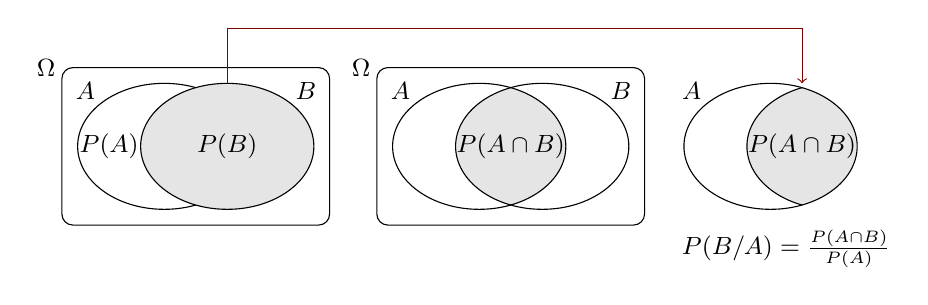
\begin{tikzpicture}[x=10mm,y=10mm,font=\small]

\def\rettangolo{-- ++(3.4,0) -- ++(0,2) -- ++(-3.4,0) -- cycle}
\def\insieme_int{-- ++(4,0) -- ++(0,3) -- ++(-4,0) -- cycle}
\def\firstcircle{(1.3,1) ellipse (1.1 and .8)}
\def\secondcircle{(2.1,1) ellipse (1.1 and .8)}
\def\thirdcircle{(5.3,1) ellipse (1.1 and .8)}
\def\fourthcircle{(6.1,1) ellipse (1.1 and .8)}
\def\fifthcircle{(9,1) ellipse (1.1 and .8)}
\def\sixthcircle{(9.8,1) ellipse (1.1 and .8)}
 %insieme1
\draw[rounded corners] (0,0) \rettangolo (-.2,2) node {$\Omega$};
\draw[->,color=Maroon] (2.1,1.8)--(2.1,2.5)--(9.4,2.5)--(9.4,1.8);
\draw \firstcircle (.6,1) node {$P(A)$} (.3,1.7) node {$A$};
\filldraw[fill=gray!20!,draw=black] \secondcircle node {$P(B)$} (3.1,1.7) node{$B$};

 \begin{scope}
     \clip \thirdcircle;
     \fill[color=gray!20!] \fourthcircle;
  \end{scope}

\draw \thirdcircle (4.3,1.7) node{$A$};
\draw \fourthcircle (5.7,1) node {$P(A \cap B)$}(7.1,1.7) node {$B$};
%insieme 2
\draw[rounded corners] (4,0) \rettangolo node at (3.8,2) {$\Omega$};
 \begin{scope}
     \clip \fifthcircle;
     \fill[color=gray!20!] \sixthcircle;
     \draw \sixthcircle (9.4,1) node {$P(A \cap B)$};
  \end{scope}

\draw \fifthcircle (8,1.7) node {$A$};
\draw (9.2,-.3) node {$P(B/A)=\frac{P(A \cap B)}{P(A)}$};
\end{tikzpicture}

\end{center}
Immaginiamo la misura della probabilità come una massa unitaria da spalmare sull'evento. La probabilità di $B$ è la quantità di massa da spalmare sull'evento $B$ in relazione allo spazio degli eventi $\wp(\Omega)$. Nell'ipotesi di ricevere un'ulteriore informazione dal verificarsi di $A$, questa informazione modifica la probabilità di $B$. L'insieme di riferimento per la probabilità di $B$ non sarà più $\wp(\Omega)$, ma $\wp(A)$ e $P(B/A)$ sarà data dal rapporto della massa spalmata tra ciò che hanno in comune $A$ e $B$ cioè $P(A\cap B)$ e la probabilità di $A$ cioè $P(A)$: $P(B/A)=\frac{P(A\cap B)}{P(A)}$.

Se $P(B/A)=P(B)$ la parte della massa unitaria spalmata su $B$ e il rapporto tra la massa spalmata sull'intersezione tra $A$ e $B$ e la massa spalmata su $A$ rimane invariata e i due eventi si dicono indipendenti.

Se $P(B/A)>P(B)$ si dice che l'evento $B$ è \emph{correlato positivamente} all'evento $A$. Cioè il verificarsi di $A$ aumenta la probabilità dell'evento $B$.

Se $P(B/A)<P(B)$ si dice che l'evento $B$ è \emph{correlato negativamente} all'evento $A$. Cioè il verificarsi di $A$ diminuisce la probabilità dell'evento $B$.
\osservazione Due eventi $A$ e $B$ tra loro incompatibili cioè tali che $P(A\cap B)=0$ sono fortemente dipendenti. Infatti, in tal caso
\[P(B/A)=\frac{P(A\cap B)}{P(A)}=\frac 0{P(A)}=0\neq P(B).\]

In genere $P(A/B)\neq P(B/A)$ in quanto le due probabilità pur avendo lo stesso numeratore hanno quasi sempre denominatore diverso: 
\[P(B/A)=\frac{P(A\cap B)}{P(A)}\neq P(A/B)=\frac{P(A\cap B)}{P(B)}.\]

Per la proprietà commutativa dell'intersezione abbiamo: $P(A\cap B)=P(B\cap A)$ quindi 
\[P(A\cap B)=P(A)\cdot P(B/A)=P(B)\cdot P(A/B).\]
%\newpage
\begin{exrig}
\begin{esempio}
Conviene scommettere alla pari che in una classe composta da 23 alunni, due persone compiano gli anni nello stesso giorno dello stesso mese?

In questo esempio non consideriamo gli anni bisestili e che la probabilità di nascere in un giorno dell'anno sia la stessa per tutti i giorni dell'anno. Scommettere alla pari significa intanto attribuire alla probabilità dell'evento $A$=``due persone sono nate lo stesso giorno dello stesso mese'' il valore di $\np{0,5}$. Se la probabilità dell'evento è maggiore di $\np{0,5}$ conviene scommettere, altrimenti no.

Anche in questo caso conviene calcolare la probabilità dell'evento complementare $P(\overline A)$, cioè la probabilità che nessuno dei 23 allievi compiano gli anni nello stesso giorno dello stesso mese. $P(\overline A)=P(\overline{A_1}\cap \overline{A_2}\cap \overline{A_3}\cap\ldots \cap \overline{A_{23}})$ dove $\overline{A_i}$ rappresenta la probabilità che il compleanno dell'$i$-esimo alunno non coincida con nessuno dei compleanni degli altri alunni.

Analizziamo alcune di queste probabilità e applichiamo il teorema delle probabilità composte: $P(\overline{A_1})=\frac{365}{365}$, $P(\overline {A_2}/\overline{A_1})=\frac{364}{365}$, $P(\overline{A_3}/(\overline{A_1}\cap \overline{A_2}))=\frac{363}{365}$, $P(\overline{A_4}/(\overline{A_1}\cap \overline{A_2}\cap \overline{A_3}))=\frac{362}{365}$, \ldots{} e così via fino ad arrivare a $P(\overline{A_{23}}/(\overline{A_1}\cap \overline{A_2}\cap \ldots \cap \overline{A_{22}}))=\frac{343}{365}$.

Il primo allievo avrà la certezza di compiere gli anni in un qualsiasi giorno dell'anno; il secondo allievo avrà una probabilità pari a 364 giorni su 365 di non compiere gli anni nello stesso giorno del primo; il terzo allievo una probabilità di 363 giorni su 365 condizionata a non compiere gli anni lo stesso giorno del primo e del secondo; e così via fino alla probabilità dell'ultimo allievo pari a 343 giorni su 365 di non compiere gli anni lo stesso giorno dei propri compagni.

Ora applichiamo il teorema delle probabilità composte: \[ P(\overline A)=\frac{365}{365}\cdot \frac{364}{365}\cdot \frac{363}{365}\cdot \ldots \cdot \frac{343}{365}=\frac{365\cdot 364\cdot 363\cdot \ldots \cdot 343}{365^{23}}=\np{0,493}=\np{49,3}\%.\] Dato che $P(A)=1-P(\overline A)=1-\np{0,493}=\np{0,507}=\np{50,7}\%$.
\conclusione Conviene scommettere alla pari sull'evento $A$.
\end{esempio}
\end{exrig}
Il problema dell'esempio precedente si può schematizzare anche come segue: in un'urna ci sono $365$ palline numerate da $1$ a $365$. Qual è la probabilità di estrarre 2 volte la stessa pallina in 23 estrazioni, rimettendo la pallina nell'urna dopo ogni estrazione?

\vspazio\ovalbox{\risolvii \ref{ese:9.60}, \ref{ese:9.61}, \ref{ese:9.62}, \ref{ese:9.63}, \ref{ese:9.64}}
\newpage
% (c)~2014 Claudio Carboncini - claudio.carboncini@gmail.com
% (c)~2014 Dimitrios Vrettos - d.vrettos@gmail.com
\section{Esercizi}
\subsection{Esercizi dei singoli paragrafi}
\subsection*{\thechapter.1 - Gli eventi}

\begin{esercizio}
 \label{ese:9.1}
Quali dei seguenti eventi sono certi, probabili, impossibili
\begin{enumeratea}
\item Il giorno di Pasquetta pioverà;
\item il giorno di Pasqua sarà domenica;
\item comprando un biglietto della lotteria vincerò il primo premio;
\item quest'anno sarò promosso;
\item il 30 febbraio sarà domenica.
\end{enumeratea}
\end{esercizio}

\begin{esercizio}
 \label{ese:9.2}
Aprendo a caso un libro di 200 pagine indica se gli eventi seguenti sono impossibili, certi o casuali e in questo ultimo caso indica se sono elementari.
\begin{enumeratea}
\item Si prenda la pagina 156: \ldots\ldots\ldots\ldots;
\item si prenda la pagina 210: \ldots\ldots\ldots\ldots;
\item si prenda una pagina minore o uguale a 200: \ldots\ldots\ldots\ldots;
\item si prenda una pagina multipla di 10: \ldots\ldots\ldots\ldots
\end{enumeratea}
\end{esercizio}

\begin{esercizio}
 \label{ese:9.3}
Completa la tabella:
\begin{center}
\begin{tabular}{lll}
Insieme / Evento & Spazio degli eventi & Numero degli eventi\\
\midrule
\multicolumn{3}{l}{Lanciando una moneta ottengo croce}\\
$E=\{\text{croce}\} $ & $ \Omega =\{$testa, croce$\} $ & $ 2^2=4 $\\
\midrule
\multicolumn{3}{l}{Lanciando un dado ottengo 1 o 6} \\
$E=\{1$, $6\}$ & $\Omega =\{1$, 2, \ldots, \ldots, \ldots, \ldots$\}$ & $ 2^6=\ldots$\\
\midrule
\multicolumn{3}{l}{Pallina con un numero primo da un'urna con 15 palline numerate da 1 a 15}\\
$E=\{2$, 3, 5, \ldots, \ldots, \ldots$\}$ & $\Omega=\{x\in \insN \mid 1\le x\le 15\}$ & $2^{15}$\\
\midrule
\multicolumn{3}{l}{Estraendo una carta da un mazzo di 40 carte, si presenta il 7 di denari}\\
$ E=\{7\text{ di denari}\} $ & $ \Omega =\{x\in A\mid A=\{\text{Mazzo da 40}\}\} $ & \ldots\ldots\ldots\ldots\\
\midrule
\multicolumn{3}{l}{Lanciando due monete ottengo facce diverse}\\
\ldots \ldots \ldots \ldots \ldots & \ldots \ldots \ldots \ldots & \ldots \ldots \ldots \ldots\\
\midrule
\multicolumn{3}{l}{Lanciando un dato ottengo un numero pari}\\
\ldots \ldots \ldots \ldots \ldots & \ldots \ldots \ldots \ldots & \ldots \ldots \ldots \ldots\\
\midrule
\multicolumn{3}{l}{Pallina con un numero multiplo di 3 da un'urna con 15 palline numerate da 1 a 15}\\
\ldots \ldots \ldots \ldots \ldots & \ldots \ldots \ldots \ldots & \ldots \ldots \ldots \ldots\\
\midrule
\multicolumn{3}{l}{Estraendo una carta da un mazzo di 40 carte, si presenta un asso}\\
\ldots \ldots \ldots \ldots \ldots & \ldots \ldots \ldots \ldots & \ldots \ldots \ldots \ldots\\
\end{tabular}
\end{center}
\end{esercizio}
%\newpage
\pagebreak
\begin{esercizio}
 \label{ese:9.4}
Estraendo una carta da un mazzo di 40 carte napoletane, individua fra le seguenti le coppie di eventi incompatibili:
\begin{multicols}{2}
\begin{enumeratea}
\item La carta estratta è un re;
\item la carta estratta è di spade.
\item la carta estratta è un 5.
\item la carta estratta è una figura.
\item la carta estratta è di denari.
\item la carta estratta è un multiplo di 3.
\item la carta estratta non è una figura.
\end{enumeratea}
\end{multicols}
Quali sono i 2 eventi la cui unione genera un evento certo?
\end{esercizio}

\begin{esercizio}
 \label{ese:9.5}
 Considerando la distribuzione dei sessi in famiglie con due figli in cui lo spazio degli eventi $\Omega =\{{M;M}$, ${M;F}$, ${F;M}$, ${F;F}\}$ quali sono l'intersezione e l'unione degli eventi $E_1$ =``Il primo figlio è maschio'' e $E_2$ = ``Il secondo figlio è maschio''.
\end{esercizio}

\subsection*{\thechapter.2 - Definizioni di probabilità}

\begin{esercizio}
 \label{ese:9.6}
Quali tra i seguenti numeri possono essere misure di probabilità? \[ \np{1,5}\text{, }\np{0,5}\text{, }25\text{, }100\%\text{, }\np{-0,1}\text{, }\frac 1 2\text{, }\frac 4 3\text{, }0\text{, }120\%\text{, }\np{0,}\overline{3}. \]
\end{esercizio}

\begin{esercizio}
 \label{ese:9.7}
Elenca i casi favorevoli all'evento: ``lanciando tre dadi la somma delle facce è 5''.
\end{esercizio}

\begin{esercizio}[\Ast]
 \label{ese:9.8}
Per uno studente è indifferente ricevere \officialeuro~$350$ senza condizioni, oppure un motorino del valore \officialeuro~$\np{1500}$ solo se sarà promosso. Qual è la probabilità che lo studente attribuisce alla sua promozione?
\end{esercizio}

\begin{esercizio}[\Ast]
 \label{ese:9.9}
Uno studente è disposto a puntare 10 € per riceverne 60 solo se sarà interrogato in matematica. Quale probabilità lo studente attribuisce all'eventualità di essere interrogato in matematica?
\end{esercizio}

\begin{esercizio}[\Ast]
 \label{ese:9.10}
Tre amici si sfidano ad una gara di scacchi. Giudico che due di essi si equivalgano, mentre ritengo che il terzo abbia probabilità doppia di ciascuno degli altri due sfidanti. Quale probabilità attribuisco a ciascuno dei tre giocatori?
\end{esercizio}

\begin{esercizio}[\Ast]
 \label{ese:9.11}
Un'urna contiene 3 palline bianche, 5 rosse e 7 verdi tutte uguali e distinguibili solo per il colore. Calcolare la probabilità che estraendo a caso una pallina dall'urna si verificano i seguenti eventi.
\begin{itemize*}
\item $ A= $ si estrae una pallina rossa;
\item $ B= $ si estrae una pallina bianca;
\item $ C= $ si estrae una pallina bianca o verde.
\end{itemize*}
\end{esercizio}

\begin{esercizio}
 \label{ese:9.12}
Si lanciano 3 monete equilibrate (testa e croce sono egualmente possibili); calcolare la probabilità di ottenere due croci e una testa.
\end{esercizio}

\begin{esercizio}[\Ast]
 \label{ese:9.13}
Calcolare la probabilità che lanciando 2 dadi regolari la somma dei numeri che si presentano sia 6.
\end{esercizio}

\begin{esercizio}[\Ast]
 \label{ese:9.14}
Un'urna contiene 100 palline identiche, numerate da 1 a 100. Calcolare la probabilità che estraendo a caso una pallina dall'urna, essa sia un multiplo di 10.
\end{esercizio}

\begin{esercizio}[\Ast]
 \label{ese:9.15}
Un'urna contiene 15 palline identiche, numerate da 1 a 15. Calcolare la probabilità che estraendo a caso due palline dall'urna, la loro somma sia 10.
\end{esercizio}

\begin{esercizio}[\Ast]
 \label{ese:9.16}
Calcola la probabilità che lanciando 4 volte una moneta equilibrata escano solo due teste.
\end{esercizio}

\begin{esercizio}[\Ast]
 \label{ese:9.17}
Pago alla mia compagnia di assicurazione un premio di \officialeuro~$450$ all'anno per avere assicurato contro il furto la mia auto che ho pagato \officialeuro~$\np{12000}$. Quale probabilità viene attribuita dalla compagnia al furto dell'auto?
\end{esercizio}

\begin{esercizio}[\Ast]
 \label{ese:9.18}
E' più facile vincere un premio acquistando un biglietto nella lotteria A che prevede 10 premi di ugual valore su un totale di $\np{5000}$ biglietti venduti o nella lotteria B che prevede 7 premi su $\np{3000}$ biglietti venduti?
Se ogni premio per entrambe le lotteria ammonta a \officialeuro~$\np{1000}$, quale dovrebbe essere un prezzo equo per la lotteria A? Quale il prezzo equo per la lotteria B?
\end{esercizio}

\begin{esercizio}
 \label{ese:9.19}
In Italia nel 2005 sono stati denunciati dalla polizia $\np{2579124}$ crimini penali, nello stesso periodo in Danimarca sono stati denunciati $\np{432704}$ crimini. Sulla base di questi dati ritieni che sia più sicuro vivere in Danimarca?
\end{esercizio}

\begin{esercizio}
 \label{ese:9.20}
 In un mazzo di 40 carte napoletane calcola la probabilità che estraendo a caso una carta essa sia:
\begin{itemize*}
\item $ A= $ un re;
\item $ B= $ una carta a denari;
\item $ C= $ una carta minore di 8;
\item $ D = $ una carta con punteggio pari.
\end{itemize*}
\end{esercizio}

\begin{esercizio}
 \label{ese:9.21}
Un mazzo di carte francesi è composto da 54 carte, 13 per seme e due jolly, i semi sono cuori e quadri di colore rosso, picche e fiori di colore nero. Calcolare la probabilità che estraendo a caso una carta
\begin{itemize*}
\item $ A= $ sia un jolly;
\item $ B= $ sia un re;
\item $ C= $ sia l'asso di picche,
\item $ D= $ sia una carta di colore rosso.
\end{itemize*}
\end{esercizio}

\begin{esercizio}
 \label{ese:9.22}
Da un mazzo di 40 carte napoletane vengono tolte tutte le figure, calcola la probabilità di estrarre una carta a denari.
\end{esercizio}

\begin{esercizio}
 \label{ese:9.23}
In un sacchetto vengono inserite 21 tessere, su ciascuna delle quali è stampata una lettera dell'alfabeto italiano. Calcola la probabilità che estraendo a caso una tessera essa sia
\begin{itemize*}
\item $ A= $ una consonante;
\item $ B= $ una vocale;
\item $ C= $ una lettera della parola MATEMATICA.
\end{itemize*}
\end{esercizio}

\begin{esercizio}
 \label{ese:9.24}
Nelle estrazioni del Lotto si estraggono dei numeri a caso compresi tra 1 e 90. Calcola la probabilità che il primo numero estratto sia:
\begin{itemize*}
\item $ A= $ il 90;
\item $ B= $ un numero pari;
\item $ C= $ un multiplo di 3;
\item $ D= $ contenga la cifra 1.
\end{itemize*}
\end{esercizio}

\begin{esercizio}
 \label{ese:9.25}
In un ipermercato si sono venduti in un anno $\np{1286}$ cellulari di tipo A e $780$ cellulari di tipo B. Mentre erano ancora in garanzia sono stati restituiti $12$ cellulari di tipo A e $11$ cellulari di tipo B perché malfunzionanti. Comprando un cellulare di tipo A, qual è la probabilità che sia malfunzionante? Qual è la probabilità che sia malfunzionante un cellulare di tipo B?
\end{esercizio}

\begin{esercizio}
 \label{ese:9.26}
Quando vado al lavoro parcheggio l'auto nei parcheggi a pagamento ma non sempre compro il biglietto del parcheggio. Precisamente lo compro il lunedì e il giovedì, non lo compro il martedì e il mercoledì, il venerdì vado sempre con l'auto di un collega, il sabato e la domenica non lavoro. Quando vado al lavoro, che probabilità ho di prendere la multa per non aver pagato il parcheggio?
\end{esercizio}

\begin{esercizio}
 \label{ese:9.27}
Un semaforo mostra il rosso per 120'', il verde per 60'', il giallo per 10''. Qual è la probabilità di incontrare il semaforo quando è verde?
\end{esercizio}

\subsection*{\thechapter.3 - Probabilità dell'unione di due eventi}

\begin{esercizio}[\Ast]
 \label{ese:9.28}
 Lanciando un dado regolare, si calcoli la probabilità che esca un numero dispari o minore di 4.
\end{esercizio}

\begin{esercizio}[\Ast]
 \label{ese:9.29}
Da un'urna che contiene 12 palline identiche, numerate da 1 a 12, se ne estrae una. Calcolare la probabilità che la pallina presenti un numero minore di 6 o un numero maggiore di 8.
\end{esercizio}

\begin{esercizio}[\Ast]
 \label{ese:9.30}
Da un'urna che contiene 12 palline, numerate da 1 a 12, se ne estrae una. Calcolare la probabilità che la pallina presenti un numero pari o un numero maggiore di 8.
\end{esercizio}

\begin{esercizio}[\Ast]
 \label{ese:9.31}
Lanciando un dado regolare, si calcoli la probabilità che esca un numero pari o minore di 2.
\end{esercizio}

\begin{esercizio}[\Ast]
 \label{ese:9.32}
Calcolare la probabilità che scegliendo a caso una carta da un mazzo di carte francesi di 54 carte si prenda una carta di picche o un re.
\end{esercizio}

\begin{esercizio}[\Ast]
 \label{ese:9.33}
Estraendo una carta da un mazzo di 40 carte, calcolare la probabilità che sia un 3 o una carta di spade.
\end{esercizio}

\begin{esercizio}[\Ast]
 \label{ese:9.34}
 Da un'urna che contiene 5 palline rosse, 8 palline blu, 12 palline bianche, 15 palline gialle, se ne estrae una. Calcolare la probabilità che la pallina sia rossa o blu o gialla.
\end{esercizio}

\begin{esercizio}[\Ast]
 \label{ese:9.35}
Da un'urna che contiene 30 palline identiche, numerate da 1 a 30, se ne estrae una. Calcolare la probabilità che il numero della pallina sia minore di 20 o multiplo di 4.
\end{esercizio}

\begin{esercizio}
 \label{ese:9.36}
Per un mazzo di 40 carte napoletane calcola la probabilità di estrarre
\begin{itemize*}
\item $ A= $ un asso o un re;
\item $ B= $ un sette o una carta a bastoni;
\item $ C= $ una figura o una carta a denari.
\end{itemize*}
\end{esercizio}

\begin{esercizio}
 \label{ese:9.37}
Calcola la probabilità che lanciando un dado a sei facce esca un numero pari o un multiplo di 3.
\end{esercizio}

\begin{esercizio}
 \label{ese:9.38}
Nel gioco della tombola si estrae una pallina numerata da un sacchetto contenente 90 palline numerate da 1 a 90. Calcola la probabilità che estraendo la prima pallina essa riporti:
\begin{itemize*}
\item $ A= $ un multiplo di 5 o un multiplo di 10,
\item $ B= $ un numero pari o un multiplo di 5,
\item $ C= $ un numero che contenga la cifra 5 o la cifra 2.
\end{itemize*}
\end{esercizio}

\subsection*{\thechapter.4 - Probabilità dell'evento complementare}

\begin{esercizio}
 \label{ese:9.39}
La seguente tabella è tratta dalla tavola di mortalità dei maschi al 2002 relativa a una popolazione di $\np{100000}$ individui:
\begin{center}
\begin{tabular}{lccccc}
Età & $ 0\le x<20 $ &$ 20\le x<40 $ & $ 40\le x<60 $ & $ 60\le x<80 $ & $ 80\le x<100 $ \\
Decessi & $997$ & $\np{1909}$ & $\np{7227}$ & $\np{39791}$ & $\np{49433}$\\
\end{tabular}
\end{center}
Calcola la probabilità per un individuo dell'età di 20 anni di vivere almeno per altri 40 anni.
\end{esercizio}

\begin{esercizio}[\Ast]
 \label{ese:9.40}
Calcola la probabilità di vincita dell'Italia ai campionati mondiali di calcio se i bookmaker scommettono su una sua vincita 5 a 12.
\end{esercizio}

\begin{esercizio}[\Ast]
 \label{ese:9.41}
In un incontro di boxe il pugile Cacine viene dato 7:1 contro il detentore del titolo Pickdur.
Secondo gli allibratori, quale la probabilità ha Cacine di conquistare il titolo?
Quali le poste per Pickdur?
\end{esercizio}

\begin{esercizio}[\Ast]
 \label{ese:9.42}
Quanto devo puntare su Celestino, che viene dato vincente 21:4 per riscuotere \officialeuro~$500$?
\end{esercizio}

\begin{esercizio}[\Ast]
 \label{ese:9.43}
Un cubo di legno viene verniciato e successivamente segato parallelamente alle facce in modo da ottenere $\np{1000}$ cubetti. Quanti tagli sono necessari? Qual è la probabilità che, una volta mescolati i cubetti, si estragga
\begin{itemize*}
\item $ A= $ un cubetto con una sola faccia verniciata;
\item $ B= $ un cubetto con due facce verniciate;
\item $ C= $ un cubetto con nessuna faccia verniciata.
\end{itemize*}
\end{esercizio}

\begin{esercizio}[\Ast]
 \label{ese:9.44}
In un circolo vi sono 100 soci. Di essi si sa che 44 sanno giocare a dama, 39 a scacchi, 8 sanno giocare sia a dama che a scacchi. Estraendo a sorte uno dei 100 soci, qual è la probabilità che sia una persona che non sappia giocare ad alcun gioco.
\end{esercizio}

\begin{esercizio}[\Ast]
 \label{ese:9.45}
Da un mazzo di 40 carte si estrae 1 carta. Calcola la probabilità dei seguenti eventi:
\begin{itemize*}
\item $ A= $ la carta non è di spade;
\item $ B= $ la carta non è una figura;
\item $ C= $ la carta non è un 2.
\end{itemize*}
\end{esercizio}

\begin{esercizio}[\Ast]
 \label{ese:9.46}
Calcola la probabilità che lanciando 4 volte una moneta equilibrata esca almeno una testa.
\end{esercizio}

\subsection*{\thechapter.5 - Probabilità dell'evento intersezione di due eventi}

\begin{esercizio}[\Ast]
 \label{ese:9.47}
Nel lancio di due monete qual è la probabilità che almeno una sia croce?
\end{esercizio}

\begin{esercizio}[\Ast]
 \label{ese:9.48}
Nel lancio di due dadi qual è la probabilità di avere un totale di 8 o due numeri uguali?
\end{esercizio}

\begin{esercizio}[\Ast]
 \label{ese:9.49}
Qual è la probabilità, nel lancio di due dadi, che la somma dei punti sia almeno 9?
\end{esercizio}

\begin{esercizio}[\Ast]
 \label{ese:9.50}
Nel lancio di due dadi, punto \officialeuro~$7$ sul fatto che la somma delle facce sia uguale a 5. Quanto devo ricevere perché il gioco sia equo?
\end{esercizio}

\begin{esercizio}[\Ast]
 \label{ese:9.51}
La probabilità che un proiettile colpisca un determinato bersaglio è $\np{0,5}$. Qual è la probabilità che tre proiettili lanciati uno dopo l'altro colpiscano tutti il bersaglio.
\end{esercizio}

\begin{esercizio}[\Ast]
 \label{ese:9.52}
Due persone giocano con le dita di entrambe le mani a pari e dispari. Con una posta 1:1 conviene giocare sul pari o sul dispari?
\end{esercizio}

\begin{esercizio}[\Ast]
 \label{ese:9.53}
Un allievo cuoco prepara la cena. La probabilità che la minestra sia troppo salata è pari a $\np{0,3}$ e che l'arrosto bruci sia pari a $\np{0,4}$. Qual è la probabilità che la cena riesca bene?
\end{esercizio}

\begin{esercizio}[\Ast]
 \label{ese:9.54}
Una scopa elettrica è formata da due apparati: il motore che si guasta una volta su 10 dopo un anno e la carrozzeria che si rompe una volta su 100 dopo un anno. Che probabilità ha la scopa elettrica di essere funzionante dopo un anno?
\end{esercizio}

\begin{esercizio}[\Ast]
 \label{ese:9.55}
Una coppia ha caratteri ereditari tali che ogni loro figlio ha probabilità pari a $1/4$ di essere malato. I genitori vorrebbero avere due figli. Calcolare la probabilità di avere:
\begin{itemize*}
\item $ A= $ entrambi i figli sani;
\item $ B= $ almeno un figlio malato.
\end{itemize*}
\end{esercizio}

\begin{esercizio}[\Ast]
 \label{ese:9.56}
Determinare la probabilità che lanciando tre volte una moneta si presentino
\begin{itemize*}
\item $ A= $ 3 Teste;
\item $ B= $ 1 Testa;
\item $ C= $ 2 Teste.
\end{itemize*}
\end{esercizio}

\begin{esercizio}[\Ast]
 \label{ese:9.57}
Nel lancio di una moneta e di un dado calcolare la probabilità di:
\begin{itemize*}
\item $ A= $ ottenere Croce e il 6;
\item $ B= $ ottenere Testa e un numero multiplo di 2;
\item $ C= $ ottenere Croce e un numero maggiore di 2.
\end{itemize*}
\end{esercizio}

\begin{esercizio}[\Ast]
 \label{ese:9.58}
In un'urna ci sono 6 palline, di cui 2 nere e 4 bianche: calcola la probabilità di estrarre palline di diverso colore nel caso in cui la prima pallina viene rimessa nell'urna.
\end{esercizio}

\begin{esercizio}
 \label{ese:9.59}
L'urna $ U_1 $ contiene 10 palline rosse e 15 bianche, l'urna $ U_2 $ contiene 12 palline rosse e 13 palline bianche. Calcola la probabilità che estraendo una pallina da $ U_1 $ e una pallina da $ U_2 $ siano entrambe rosse.
\end{esercizio}

\begin{esercizio}[\Ast]
 \label{ese:9.60}
 Un'urna contiene 10 palline rosse, 7 palline nere e 2 bianche. Estraendone simultaneamente tre, calcolare la probabilità:
\begin{itemize*}
 \item $ A= $ tutte e tre rosse;
 \item $ B= $ tutte e tre bianche;
 \item $ C= $ 1 rossa e 2 nere;
 \item $ D= $ tutte di colore diverso;
 \item $ E= $ una sola bianca.
\end{itemize*}
\end{esercizio}

\begin{esercizio}[\Ast]
 \label{ese:9.61}
 Da un mazzo di 40 carte, si estrae una carta a caso. Determina la probabilità:
\begin{itemize*}
\item $ A= $ che esca un Re;
\item $ B= $ che esca un Re nell'ipotesi che sia uscita una figura;
\item $ C= $ che esca un Re nell'ipotesi che sia uscito il seme di fiori;
\item $ D= $ che esca il seme di fiori dopo che è uscito un Re.
\end{itemize*}
Tra gli eventi $A$, $B$, $C$ e $D$, quali sono indipendenti?
\end{esercizio}

\begin{esercizio}[\Ast]
 \label{ese:9.62}
Uno studente universitario ha la probabilità $\np{0,3}$ di superare l'esame di matematica e $\np{0,5}$ di superare l'esame di diritto privato. Se i due eventi sono indipendenti determinare la probabilità che lo studente ha di superare
\begin{itemize*}
\item $ A= $ tutti e due gli esami;
\item $ B= $ almeno un esame.
\end{itemize*}
\end{esercizio}

\begin{esercizio}[\Ast]
 \label{ese:9.63}
Un'urna contiene 5 palline bianche e 12 nere. Estraendole due a caso qual è la probabilità che siano dello stesso colore?
\end{esercizio}

\begin{esercizio}[\Ast]
 \label{ese:9.64}
Uno studente ha la probabilità del $55\%$ di prendere il debito in matematica, del $30\%$ di prendere il debito in inglese e del $20\%$ di prendere il debito in entrambe le materie. Valutare la probabilità di:
\begin{itemize*}
\item $ A= $ avere il debito in matematica nell'ipotesi di averlo già preso in inglese;
\item $ B= $ avere il debito in inglese nell'ipotesi di averlo già preso in matematica;
\item $ C= $ avere il debito in matematica nell'ipotesi di non averlo preso in inglese;
\item $ D= $ avere il debito in inglese nell'ipotesi di non averlo preso in matematica;
\item $ E= $ non avere il debito in matematica nell'ipotesi di averlo preso in inglese;
\item $ F= $ non avere il debito in inglese nell'ipotesi di non averlo preso in matematica.
\end{itemize*}
\end{esercizio}

\subsection*{Esercizi dalle prove Invalsi}

\begin{esercizio}[Prove Invalsi~2005]% \label{ese:9.65}
Se si lanciano contemporaneamente due monete, qual è la probabilità che escano una testa e una croce?
\end{esercizio}

\begin{esercizio}[Prove Invalsi~2005] % \label{ese:9.66}
Qual è la probabilità che su 6 lanci di un comune dado a 6 facce, non truccato, si abbia per 6 volte il numero 3?
\end{esercizio}

\begin{esercizio} [Prove Invalsi~2005]% \label{ese:9.67}
Un'urna contiene 20 gettoni numerati da 1 a 20. Si estrae un gettone: è un numero pari. Senza reinserire il gettone, se ne estrae un secondo. Qual è la probabilità di estrarre un numero dispari?
\end{esercizio}

\begin{esercizio}[Prove Invalsi~2006] % \label{ese:9.68}
Se lanci un dado una sola volta, quale probabilità hai di ottenere un numero pari minore di 6?
\end{esercizio}

\begin{esercizio} [Prove Invalsi~2006]% \label{ese:9.69}
È lanciato un dado non truccato a forma di ottaedro (solido regolare a otto facce), le cui facce sono numerate da 1 a 8. Qual è la probabilità che esca una faccia il cui numero è multiplo di 3?
\end{esercizio}

\begin{esercizio} [Prove Invalsi~2006]% \label{ese:9.70}
Un mazzo di carte da poker è composto da 52 pezzi, 12 dei quali sono figure. Pescando a caso una carta, qual è la probabilità che si verifichi l'evento: ``esce una figura o un asso''?
\end{esercizio}

\begin{esercizio}[Prove Invalsi~2006] % \label{ese:9.71}
Un'urna contiene 50 gettoni colorati. 20 sono di colore verde, 18 di colore rosso, 10 di colore blu. Qual è la probabilità di pescare un gettone che non sia né verde, né rosso e né blu?
\end{esercizio}

\begin{esercizio} [Prove Invalsi~2006]% \label{ese:9.72}
La probabilità di estrarre una pallina rossa da un'urna contenente 100 palline è $3/50$. Quante sono le palline rosse contenute nell'urna?
\end{esercizio}

\begin{esercizio} [Prove Invalsi~2005]% \label{ese:9.73}
Si lancia un comune dado a 6 facce, non truccato, per 8 volte. Qual è la probabilità che al terzo lancio esca il numero 5?
\end{esercizio}

\begin{esercizio} [Prove Invalsi~2005]% \label{ese:9.74}
Data un'urna contenente 30 palline, di cui 6 rosse, 9 gialle, 3 verdi e 12 blu, quale delle seguenti affermazioni è falsa? La probabilità di estrarre una pallina \ldots
\begin{itemize*}
\item rossa o gialla è $\np{0,5}$;
\item verde è $\np{0,1}$;
\item blu o gialla è $\np{0,7}$;
\item rossa o blu è $\np{0,4}$.
\end{itemize*}
\end{esercizio}

\begin{esercizio}[Prove Invalsi~2006] % \label{ese:9.75}
Se i lanciano contemporaneamente due monete, qual è la probabilità che esca almeno una testa?
\end{esercizio}

\begin{esercizio}[Prove Invalsi~2006] % \label{ese:9.76}
Un'urna contiene 20 palline: 4 bianche, 6 rosse e 10 verdi. Quanto vale il rapporto fra la probabilità di estrarre una pallina bianca o rossa e la probabilità di estrarre una pallina rossa o verde?
\end{esercizio}

\begin{esercizio} [Prove Invalsi~2006]% \label{ese:9.77}
La probabilità di estrarre una pallina bianca da un'urna è $4/10$. Quale delle seguenti affermazioni è compatibile con la precedente?
\begin{itemize*}
\item l'urna contiene 20 palline bianche, 15 rosse e 5 nere;
\item l'urna contiene 40 palline bianche, 40 rosse e 40 nere;
\item l'urna contiene 40 palline bianche e 100 rosse;
\item l'urna contiene 80 palline bianche, 50 rosse e 70 nere.
\end{itemize*}
\end{esercizio}

\begin{esercizio}[Prove Invalsi~2006] % \label{ese:9.78}
In un dado truccato avente le facce numerate da 1 a 6, la probabilità di uscita di un numero è direttamente proporzionale al numero stesso. Quanto vale la probabilità che, lanciando il dado, esca il numero 5?
\end{esercizio}

\begin{esercizio}[Prove Invalsi~2007] % \label{ese:9.79}
Da un'urna contenente 50 palline, Marco ne estrae 20 senza rimetterle nell'urna ed osserva che 10 sono nere e 10 sono rosse. Estraendo una 21-esima pallina, qual è la probabilità che questa si nera?
\end{esercizio}

\begin{esercizio}[Prove Invalsi~2007] % \label{ese:9.80}
Quanto vale la probabilità che una persona risponda correttamente ad una domanda che prevede solo una risposta esatta, scegliendo a caso una risposta fra le quattro proposte?
\end{esercizio}

\begin{esercizio}[Prove Invalsi~2007] % \label{ese:9.81}
Un'urna contiene 21 palline, ognuna delle quali è contrassegnata da una lettera dell'alfabeto italiano. Qual è la probabilità che, estraendo a caso una di queste palline, si verifichi l'evento ``esce la lettera $\pi $''?
\end{esercizio}

\begin{esercizio} [Prove Invalsi~2007]% \label{ese:9.82}
In una lotteria i 4 premi sono assegnati per estrazioni successive, partendo dal 1° fino al 4°. Pietro ha acquistato uno solo dei 100 biglietti venduti. Egli è presente all'estrazione dei premi e l'estrazione del 1° premio lo vede perdente. Qual è la probabilità che Pietro vinca il 2° premio?
\end{esercizio}

\begin{esercizio}[Prove Invalsi~2007] % \label{ese:9.83}
Si lanciano due dadi ed escono due numeri il cui prodotto è 6. Qual è la probabilità che uno dei due numeri usciti sia 2?
\end{esercizio}

\begin{esercizio} [Prove Invalsi~2007]% \label{ese:9.84}
Quanti casi possibili si ottengono gettando un dado e una moneta contemporaneamente?

A. 12 \quad B. 8 \quad C. 36 \quad D. 2 \quad E. La risposta esatta non è tra quelle proposte.
\end{esercizio}

\begin{esercizio}[Prove Invalsi~2003] % \label{ese:9.85}
 Se lanci un normale dado numerato da 1 a 6, ciascun numero ha probabilità $1/6$ di uscire. In 4 lanci successivi sono usciti i numeri 2, 3, 4 e 3. Se lanci il dado una quinta volta, qual è la probabilità che esca 3?
\begin{itemize*}
\item Maggiore di $1/6$, perché nei 4 tiri precedenti il punteggio 3 è uscito 2 volte su 4;
\item $1/6$, perché il dado non si ricorda degli eventi passati;
\item minore di $1/6$, perché il punteggio 3 è già uscito e ora è più probabile che escano gli altri;
\item $1/2$, come indica il calcolo dei casi favorevoli (due) sul totale dei casi (quattro);
\item le informazioni date non consentono di rispondere.
\end{itemize*}
\end{esercizio}

\begin{esercizio} [Prove Invalsi~2003]% \label{ese:9.86}
 Estrarre da un mazzo di carte francesi (52 carte) una carta di seme nero e figura è \ldots
\begin{itemize*}
\item più probabile che estrarre una carta di seme nero;
\item più probabile che estrarre una figura di qualunque seme;
\item meno probabile che estrarre una carta di seme nero e asso;
\item altrettanto probabile che estrarre una carta di seme nero o figura;
\item altrettanto probabile che estrarre una carta di seme rosso e figura. (Prove Invalsi 2003)
\end{itemize*}
\end{esercizio}

\begin{esercizio}[Prove Invalsi~2003] % \label{ese:9.87}
La probabilità di estrarre un 6 o un 8 da un mazzo di carte napoletane (40 carte) è \ldots
\end{esercizio}

\begin{esercizio} [Prove Invalsi~2003]% \label{ese:9.88}
Aldo e Luigi giocano a testa o croce, ciascuno di essi lancia due monete. Qual è la probabilità che il numero di teste di Luigi sia uguale a quelle ottenute da Aldo?
\end{esercizio}

\begin{esercizio} [Prove Invalsi~2004]% \label{ese:9.89}
Se lanci una normale moneta, Testa e Croce hanno entrambe probabilità $1/2$ di uscire. In 4 lanci successivi, sono usciti Testa, Croce, Testa, Testa. Se lanci la moneta una quinta volta, qual è la probabilità che esca Testa?
\begin{itemize*}
\item Maggiore di $ \frac 1 2 $;
\item uguale a $ \frac 1 2 $;
\item minore di $ \frac 1 2 $;
\item le informazioni date non consentono di rispondere.
\end{itemize*}
\end{esercizio}

\begin{esercizio} [Prove Invalsi~2004]% \label{ese:9.90}
Nel gioco della tombola qual è la probabilità di estrarre un numero maggiore di 20 e minore di 35?
\end{esercizio}

\begin{esercizio} [Prove Invalsi~2004]% \label{ese:9.91}
Qual è la probabilità che lanciando un dado esca un numero dispari o multiplo di 3?
\end{esercizio}

\subsection{Risposte}
\begin{multicols}{2}

\paragraph{\thechapter.8.} $P(E)=\np{0,23}$.

\paragraph{\thechapter.9.} $P(E)=\np{0,17}$.

\paragraph{\thechapter.10.} $P(A)=P(B)=\np{0,25}$; $P(C)=\np{0,50}$.

\paragraph{\thechapter.11.} $ P(A)=\frac{1}{3}$; $P(B)=\frac{1}{5}$; $P(C)=\frac{2}{3} $.

\paragraph{\thechapter.13.} $P(E)=\frac 5{36}$.

\paragraph{\thechapter.14.} $P(E)=\frac{10}{100}=\frac 1{10}$.

\paragraph{\thechapter.15.} $P(E)=\frac 8{210}=\frac 4{105}$

\paragraph{\thechapter.16.} $P(E)=\frac 3 8$.

\paragraph{\thechapter.17.} $P(E)=\np{0,0375}$.

\paragraph{\thechapter.18.} Biglietto B; Prezzo(A)=\officialeuro~$2$;\protect\\ Prezzo(B)=\officialeuro~$\np{2,23}$.

\paragraph{\thechapter.28.} $P(E)=\frac 2 3$.

\paragraph{\thechapter.29.} $P(E)=\frac 3 4$.

\paragraph{\thechapter.30.} $P(E)=\frac 2 3$.

\paragraph{\thechapter.31.} $P(E)=\frac 2 3$.

\paragraph{\thechapter.32.} $P(E)=\frac 8{27}$.

\paragraph{\thechapter.33.} $P(E)=\frac{13}{40}$.

\paragraph{\thechapter.34.} $P(E)=\frac 7{10}$.

\paragraph{\thechapter.35.} $P(E)=\frac{11}{15}$.

\paragraph{\thechapter.39.} $P(E)=\np{0,91}$.

\paragraph{\thechapter.40.} $P(E)=\np{0,71}$.

\paragraph{\thechapter.41.} $P(A)=\frac 1 8;B=7:1$.

\paragraph{\thechapter.42.} \officialeuro~$80$.

\paragraph{\thechapter.43.} $P(A)=\np{0,384}$; $P(B)=\np{0,096}$; $P(C)=\np{0,512}$.

\paragraph{\thechapter.44.} $P(E)=\np{0,25}$.

\paragraph{\thechapter.45.} $P(A)=\frac 3 4$; $P(B)=\frac 7{10}$; $P(C)=\frac 9{10}$.

\paragraph{\thechapter.46.} $P(E)=1-\frac 1{16}=\frac{15}{16}$.

\paragraph{\thechapter.47.} $P(E)=\frac 3 4$.

\paragraph{\thechapter.48.} $P(E)=\frac 5{18}$.

\paragraph{\thechapter.49.} $P(E)=\frac{15}{18}$.

\paragraph{\thechapter.50.} \officialeuro~$63$.

\paragraph{\thechapter.51.} $P(E)=\np{0,125}$.

\paragraph{\thechapter.52.} indifferente.

\paragraph{\thechapter.53.} $P(E)=\np{0,42}$.

\paragraph{\thechapter.54.} $P(E)=\np{89,1}\%$

\paragraph{\thechapter.55.} $ P(A)=\frac 9 {16}$; $P(B)=\frac 7 {16} $.

\paragraph{\thechapter.56.} $ P(A)=\frac 1 8$; $P(B)=\frac3 8$; $P(C)=\frac 3 8 $.

\paragraph{\thechapter.57.} $ P(A)=\frac 1 {12}$; $P(B)=\frac1 4$; $P(C)=\frac 1 3 $.

\paragraph{\thechapter.58.} $ P(E)=\frac 4 9 $.

\paragraph{\thechapter.60.} $P(A)=\np{0,12}$; $P(B)=0$; $P(C)=\np{0,22}$; $P(D)=\np{0,14}$; $P(E)=\np{0,28}$.

\paragraph{\thechapter.61.} $ P(A)=\frac 1{10}$; $ P(B)=\frac 1 3 $; $ P(C)=\frac 1{10} $; $ P(D)=\frac 1 4 $; $A$ e $C$.

\paragraph{\thechapter.62.} $P(A)=\np{0,15}$; $P(B)=\np{0,65}$.

\paragraph{\thechapter.63.} $P(A)=\np{0,56}$.

\paragraph{\thechapter.64.} $P(A)=67\%$; $P(B)=36\%$; $P(C)=50\%$; $P(D)=22\%$; $P(E)=33\%$; $P(F)=64\%$.
\end{multicols}

\cleardoublepage
